\phantomsection\addcontentsline{toc}{section}{\numberline {}CHƯƠNG 3. THIẾT KẾ CHUYỂN ĐỔI PDM SANG PCM NHIỀU GIAI ĐOẠN VÀ KIỂM THỬ BẰNG PHẦN MỀM}
\section*{CHƯƠNG 3. THIẾT KẾ CHUYỂN ĐỔI PDM SANG PCM NHIỀU GIAI ĐOẠN VÀ KIỂM THỬ BẰNG PHẦN MỀM} \label{chuong3}
\setcounter{section}{3}
\setcounter{subsection}{0}
\setcounter{figure}{0}
\setcounter{table}{0}
Ở \hyperref[chuong2]{chương 2}, chúng ta đã trình bày thảo luận về bộ chuyển đổi Sigma-Delta, phổ của tín hiệu PDM từ micro, các bộ lọc khác nhau và cách tìm ra các hệ số phù hợp cho các bộ lọc đó. Chương này mô tả các yêu cầu thiết kế, cách kết hợp tất cả lại với nhau, tạo ra bộ chuyển đổi PDM sang PCM nhiều giai đoạn và kiểm thử thiết kế bằng ngôn ngữ \textit{Python}.
\subsection{Tổng quan về hệ thống xử lý âm thanh số sử dụng MEMS Microphone}
Hình \ref{audio_top} mô tả một hệ thông xử lý âm thanh cơ bản sử dụng PDM MEMS microphone. Tín hiệu tương tự sau khi thu bằng micro sẽ được điều chế thành tín hiệu số dạng PDM - biểu diễn bằng 1 bit và tốc độ lấy mẫu cao. Để phân tích và tái tạo lại âm thanh thu được chúng ta phải đưa tín hiệu đó vào một hệ thống xử lý âm thanh số. Bộ PDM2PCM có vai trò chuyển đổi tín hiệu PDM sang PCM, sau đó bộ DSP sẽ điều chỉnh, cân bằng lại để nâng cao hiệu suất. Để âm thanh được phát trực tiếp ra loa, tín hiệu phải được đưa về dạng tương tự thông qua bộ chuyển đổi số tương tự (Audio-Codec) và bộ khuếch đại tín hiệu.
\begin{figure}[H]
    \centering
    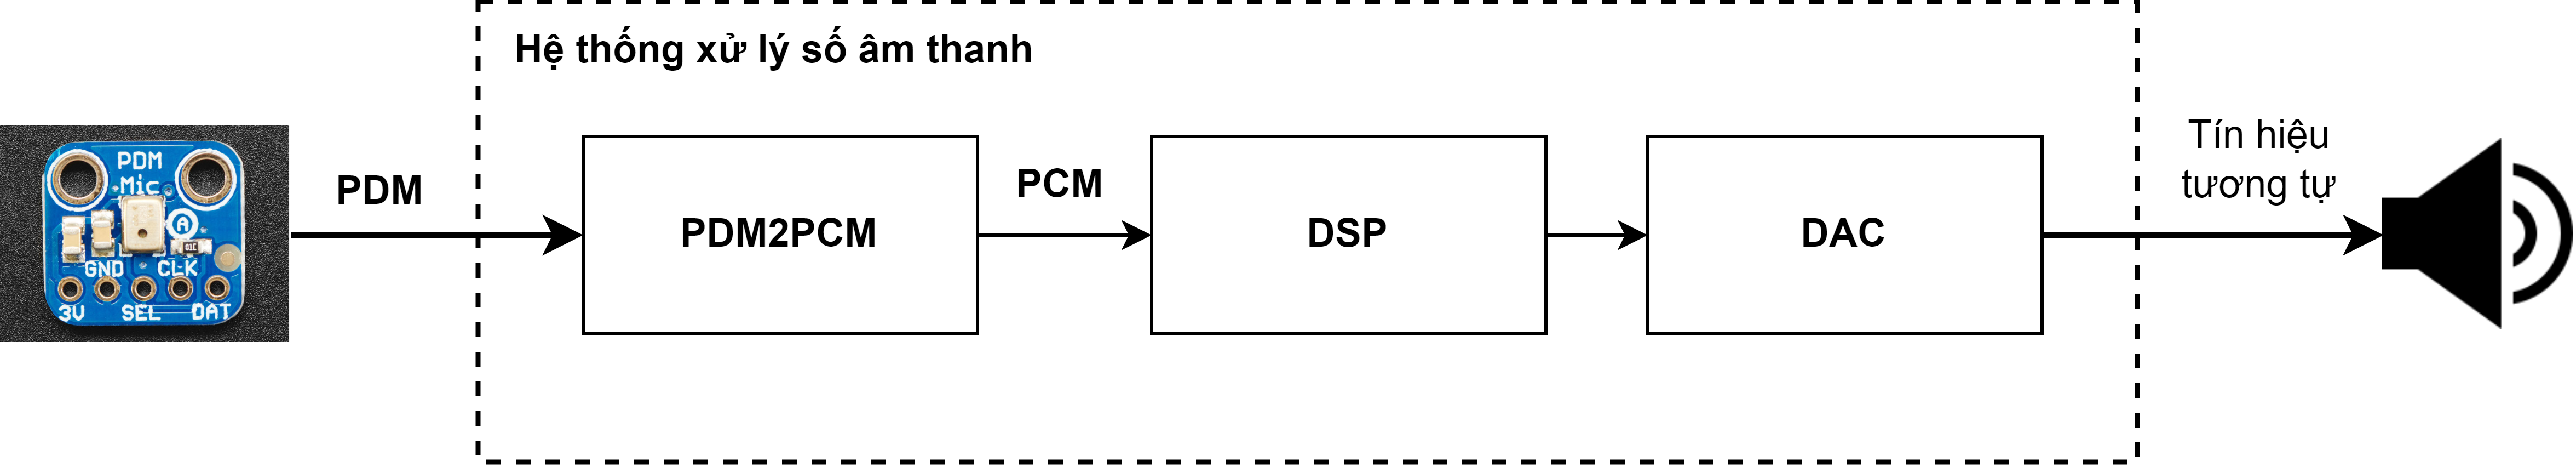
\includegraphics[width=14cm]{Images/Chuong3/MoDau/audio_top.png}
    \caption[Sơ đồ tổng quát của bộ chuyển đổi]{\bfseries \fontsize{12pt}{0pt}\selectfont Mô hình xử lý âm thanh số sử dụng MEMS Microphone}
    \label{audio_top}
\end{figure}

Ngoài cách xử lý trực tiếp như trên, tín hiệu PCM sau khi được chuyển đổi có thể lưu trữ lại, dễ dàng truyển tải và xử lý bằng phần mềm chuyên biệt trên máy tính.

\subsection{Bộ chuyển đổi đã thương mại hóa}
\noindent\textbf{Analog Devices - ADAU7112} \label{adauref}

IC ADAU7112 có chức năng chuyển đổi các luồng bít PDM âm thanh nổi thành 1 một luồng PCM. Nguồn dữ liệu PDM đầu vào có thể từ 2 microphone (trái, phải) hoặc các nguồn PDM khác. Dữ liệu PCM được đưa ra trên một cổng giao diện âm thanh nối tiếp là I2S (Inter-IC Serial) hoặc TDM (Time Domain Multiplexed). \cite{adau7112}

Hình \ref{adau7112_f} mô tả sơ đồ khối của ADAU7112. Tín hiệu PDM được đưa vào \textbf{PDM\_DAT} cũng với clock lấy mẫu (\textbf{PDM\_CLK}). Tín hiệu sau đó đưa qua bộ lọc Decimation để trích suất ra tín hiệu dạng PCM với tỷ lệ 64x. Giao thức I2S/TDM giúp đưa PCM dạng song song thành tín hiệu dạng nối tiếp để truyền tín hiệu âm thanh cho các mạch tích hợp khác thông qua cổng (\textbf{BCLK}, \textbf{FSYNC}, \textbf{SDATA}).

\begin{figure}[H]
    \centering
    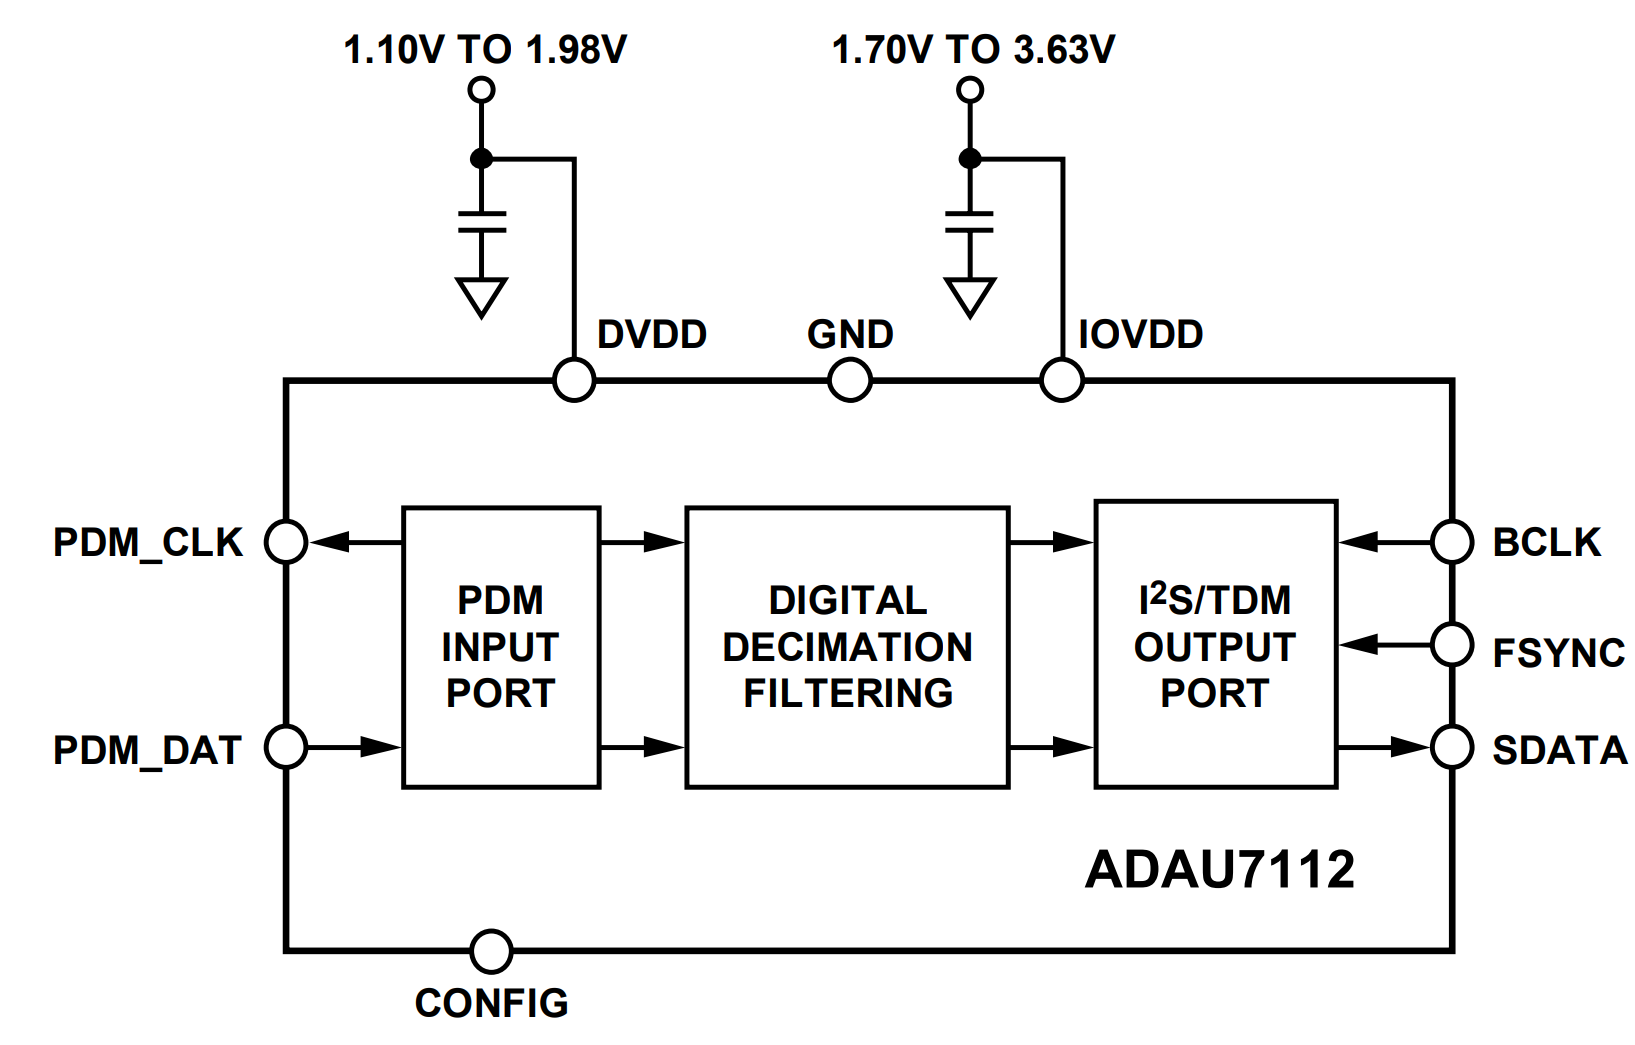
\includegraphics[width=12cm]{Images/Chuong3/MoDau/adau7112.png}
    \caption[Sơ đồ tổng quát của bộ chuyển đổi]{\bfseries \fontsize{12pt}{0pt}\selectfont Sơ đồ khối của ADAU7112}
    \label{adau7112_f}
\end{figure}

Sau đây là các thông số kỹ thuật của ADAU7112:
\begin{itemize}
    \item Số kênh PDM đầu vào: 2 kênh
    \item Tự động tạo clock PDM
    \item Tỷ số Decimation (PDM sang PCM): 64x
    \item Độ rộng của PCM: 24 bit
    \item Tốc độ lấy mẫu đầu vào (PDM): 3.072 MHz - 6.144 MHz
    \item Tốc độ lấy mẫu đầu ra: 9 kH - 96 kHz
    \item Độ suy hao giải dừng: 75 dB
    \item Điện áp hoạt động: 1.70 - 3.63 V
\end{itemize}
\subsection{Mô hình bộ chuyển đổi PDM sang PCM} \label{mohinhpdm2pcm}
Khi chúng ta quan sát phổ của tín hiệu PDM, các nhiễu lượng tử sẽ được dồn sang ở tần số cao, còn phần cần lấy thông tin sẽ ở trong một khoảng tần số thấp nhất định. Cho nên, bộ chuyển đổi sẽ chỉ cần 2 bước cơ bản (hình \ref{pdm2pcm_top}):
\begin{enumerate}
    \item Gửi tín hiệu PDM thông qua một bộ lọc thông thấp. Nó sẽ loại bỏ tất cả các nhiễu ở tần số cao.
    \item Sử dụng kỹ thuật Decimation (hạ tần) để các mẫu được lấy mẫu với tỷ lệ thấp hơn. Việc sử dụng bộ lọc thông thấp từ bước 1 cũng sẽ giúp tránh được hiện tượng chồng phổ.
\end{enumerate}

\begin{figure}[H]
    \centering
    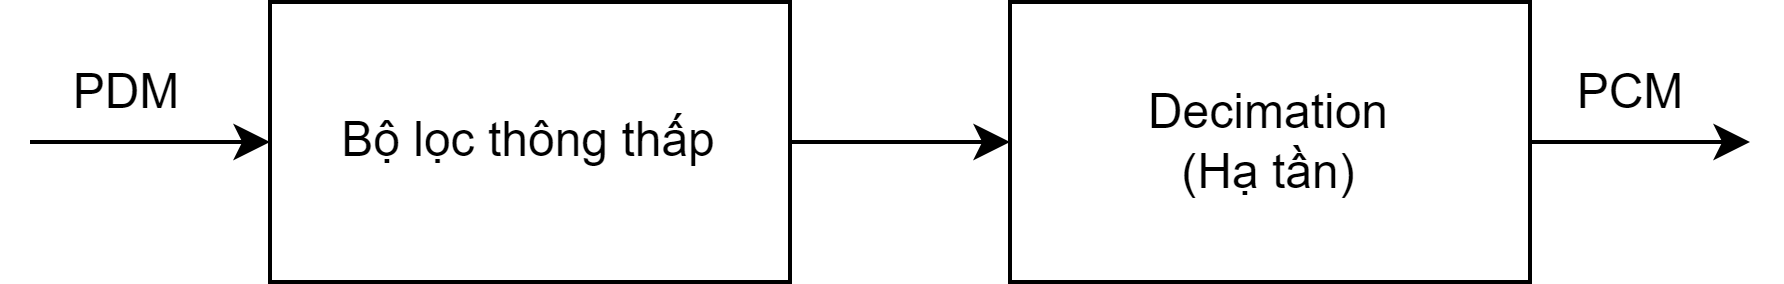
\includegraphics[width=12cm]{Images/Chuong3/pdm2pcm_top.png}
    \caption[Sơ đồ tổng quát của bộ chuyển đổi]{\bfseries \fontsize{12pt}{0pt}\selectfont Sơ đồ tổng quát của bộ chuyển đổi}
    \label{pdm2pcm_top}
\end{figure}

Như vậy, việc thiết kế bộ chuyển đổi chỉ tập trung vào chọn các thông số (dải thông, dải dừng, độ gợn sóng, độ suy hao) của bộ lọc thông thấp và tỷ số Decimation phù hợp.


\subsection{Từ thông số của Microphone đến yêu cầu thiết kế} \label{spec_muc}

MEMS Microphone (MicroelectromechanicalSystem Microphone) - thiết bị này có thể được tìm thấy phổ biến trên các điện thoại di động, các máy ghi âm hoặc các thiết bị thu thanh không sử yêu cầu về chất lượng âm thanh quá cao nhưng giá thành rẻ và phù hợp với yêu cầu sử dụng.
Ở đây, chúng ta sẽ phân tích thiết bị \textbf{MP34DT01-M} của hãng \textbf{ST}.
Về cơ bản chúng ta chỉ cần chú ý những thống số ở trên bảng \ref{datasheet}.
\begin{table}[h!] 
\centering
\caption[Các thông số kỹ thuật cần chú ý của MP34DT01-M ]{\bfseries\fontsize{12pt}{0pt}\selectfont Các thông số kỹ thuật cần chú ý của MP34DT01-M}
\begin{tabular}{|l|l|l|l|l|l|l|}
\hline
Ký hiệu & Thông tin                                                        & Min. & Typ. & Max. & Đơn vị & Ghi chú \\ \hline
AOP     & \begin{tabular}[c]{@{}l@{}}Điểm quá tải \\ âm thanh\end{tabular} &      & 120  &      & dBSPL  &         \\ \hline
SNR & \begin{tabular}[c]{@{}l@{}}Tỷ số tín hiệu\\  trên nhiễu\end{tabular} &  & 61 &  & dB & \begin{tabular}[c]{@{}l@{}}Đo ở điều\\ kiện 1kHz,\\ áp suất 1Pa\end{tabular} \\ \hline
Clock   & Tần số đầu vào                                                   & 1    & 2.4  & 3.25 & MHz    &         \\ \hline
\end{tabular}
\label{datasheet}
\end{table}

\noindent\textbf{Điểm quá tải âm thanh (AOP - Acoustic Overload Point)}: sóng hình sin 1kHz lớn nhất mà nó ít nhiều có thể ghi lại một cách đáng tin cậy.
\begin{equation} \label{dynamic}
    \text{Dynamic Range} = AOP - 94dBSPL + SNR
\end{equation}

\noindent\textbf{Dải động - Dynamic Range} được biểu diễn bằng công thức \ref{dynamic}. Với trường hợp của micro này, Dynamic Range$ = 120 -94 + 61 = 87dB$ và đây cũng là chính xác $SNR$ đầu ra của micro.

Độ suy hao dải dừng của bộ lọc sẽ được tính theo công thức \ref{stopband} \cite{pdm2pcm} và bằng 89 dB.
\begin{equation} \label{stopband}
    A_{stop band} = -3dB - 10log_{10}{(10^{-\displaystyle\frac{SNR_{after}}{10}}-10^{-\displaystyle\frac{SNR_{before}}{10}})}
\end{equation}

\noindent \textbf{Nhận xét}: Với tốc độ lấy mẫu của đầu ra 48 kHz (âm thanh chất lượng cao) và hệ số Decimation của ADAU7122 (mục \ref{adauref}) là 64 thì tần số lẫy mẫu PDM sẽ là 3072 kHz (48 kHz $\times$ 64) thỏa mãn với yêu cầu dải tần số lấy mẫu PDM của microphone. Tuy nhiên về độ suy hao dải dừng sẽ không đáp ứng được với yêu cầu của bộ lọc (89 dB > 75 dB), cho nên việc sử dụng ADAU7122 cho ứng dụng này là không khả thi.

Vì lý do trên chúng ta sẽ đề xuất một thiết kế đáp ứng được các thông số của microphone \textbf{MP34DT01-M} đã giới thiệu ở trên. Và đặc biệt, có thể thay đổi các tham số để phù hợp với mọi loại microphone cụ thể.

Bộ chuyển đổi (bộ lọc Decimation) phải đáp ứng được những yêu cầu sau:
\begin{itemize}
    \item Tốc độ lấy mẫu ở đầu ra (PCM) là 48 kHz.\\
    Tốc độ lấy mẫu 48 kHz là tốc độ phổ biến dùng cho các âm thanh chất lượng cao
    \item Tốc độ lấy mẫu PDM là 2.304 MHz.\\
    Micrô hỗ trợ tốc độ xung nhịp PDM trong khoảng từ 1 đến 3,25 MHz. Có các bộ lọc rất hiệu quả cho phép Decimation 2x, vì vậy nên chọn một tỷ lệ decimation là một số chia hết cho lũy thừa của 2. Tỷ lệ 48x được cho là phù hợp nhất.

    \item Độ gợn sóng là 0.1 dB: yêu cầu cần thiết đối với âm thanh chất lượng cao.

\begin{figure}[H]
    \centering
    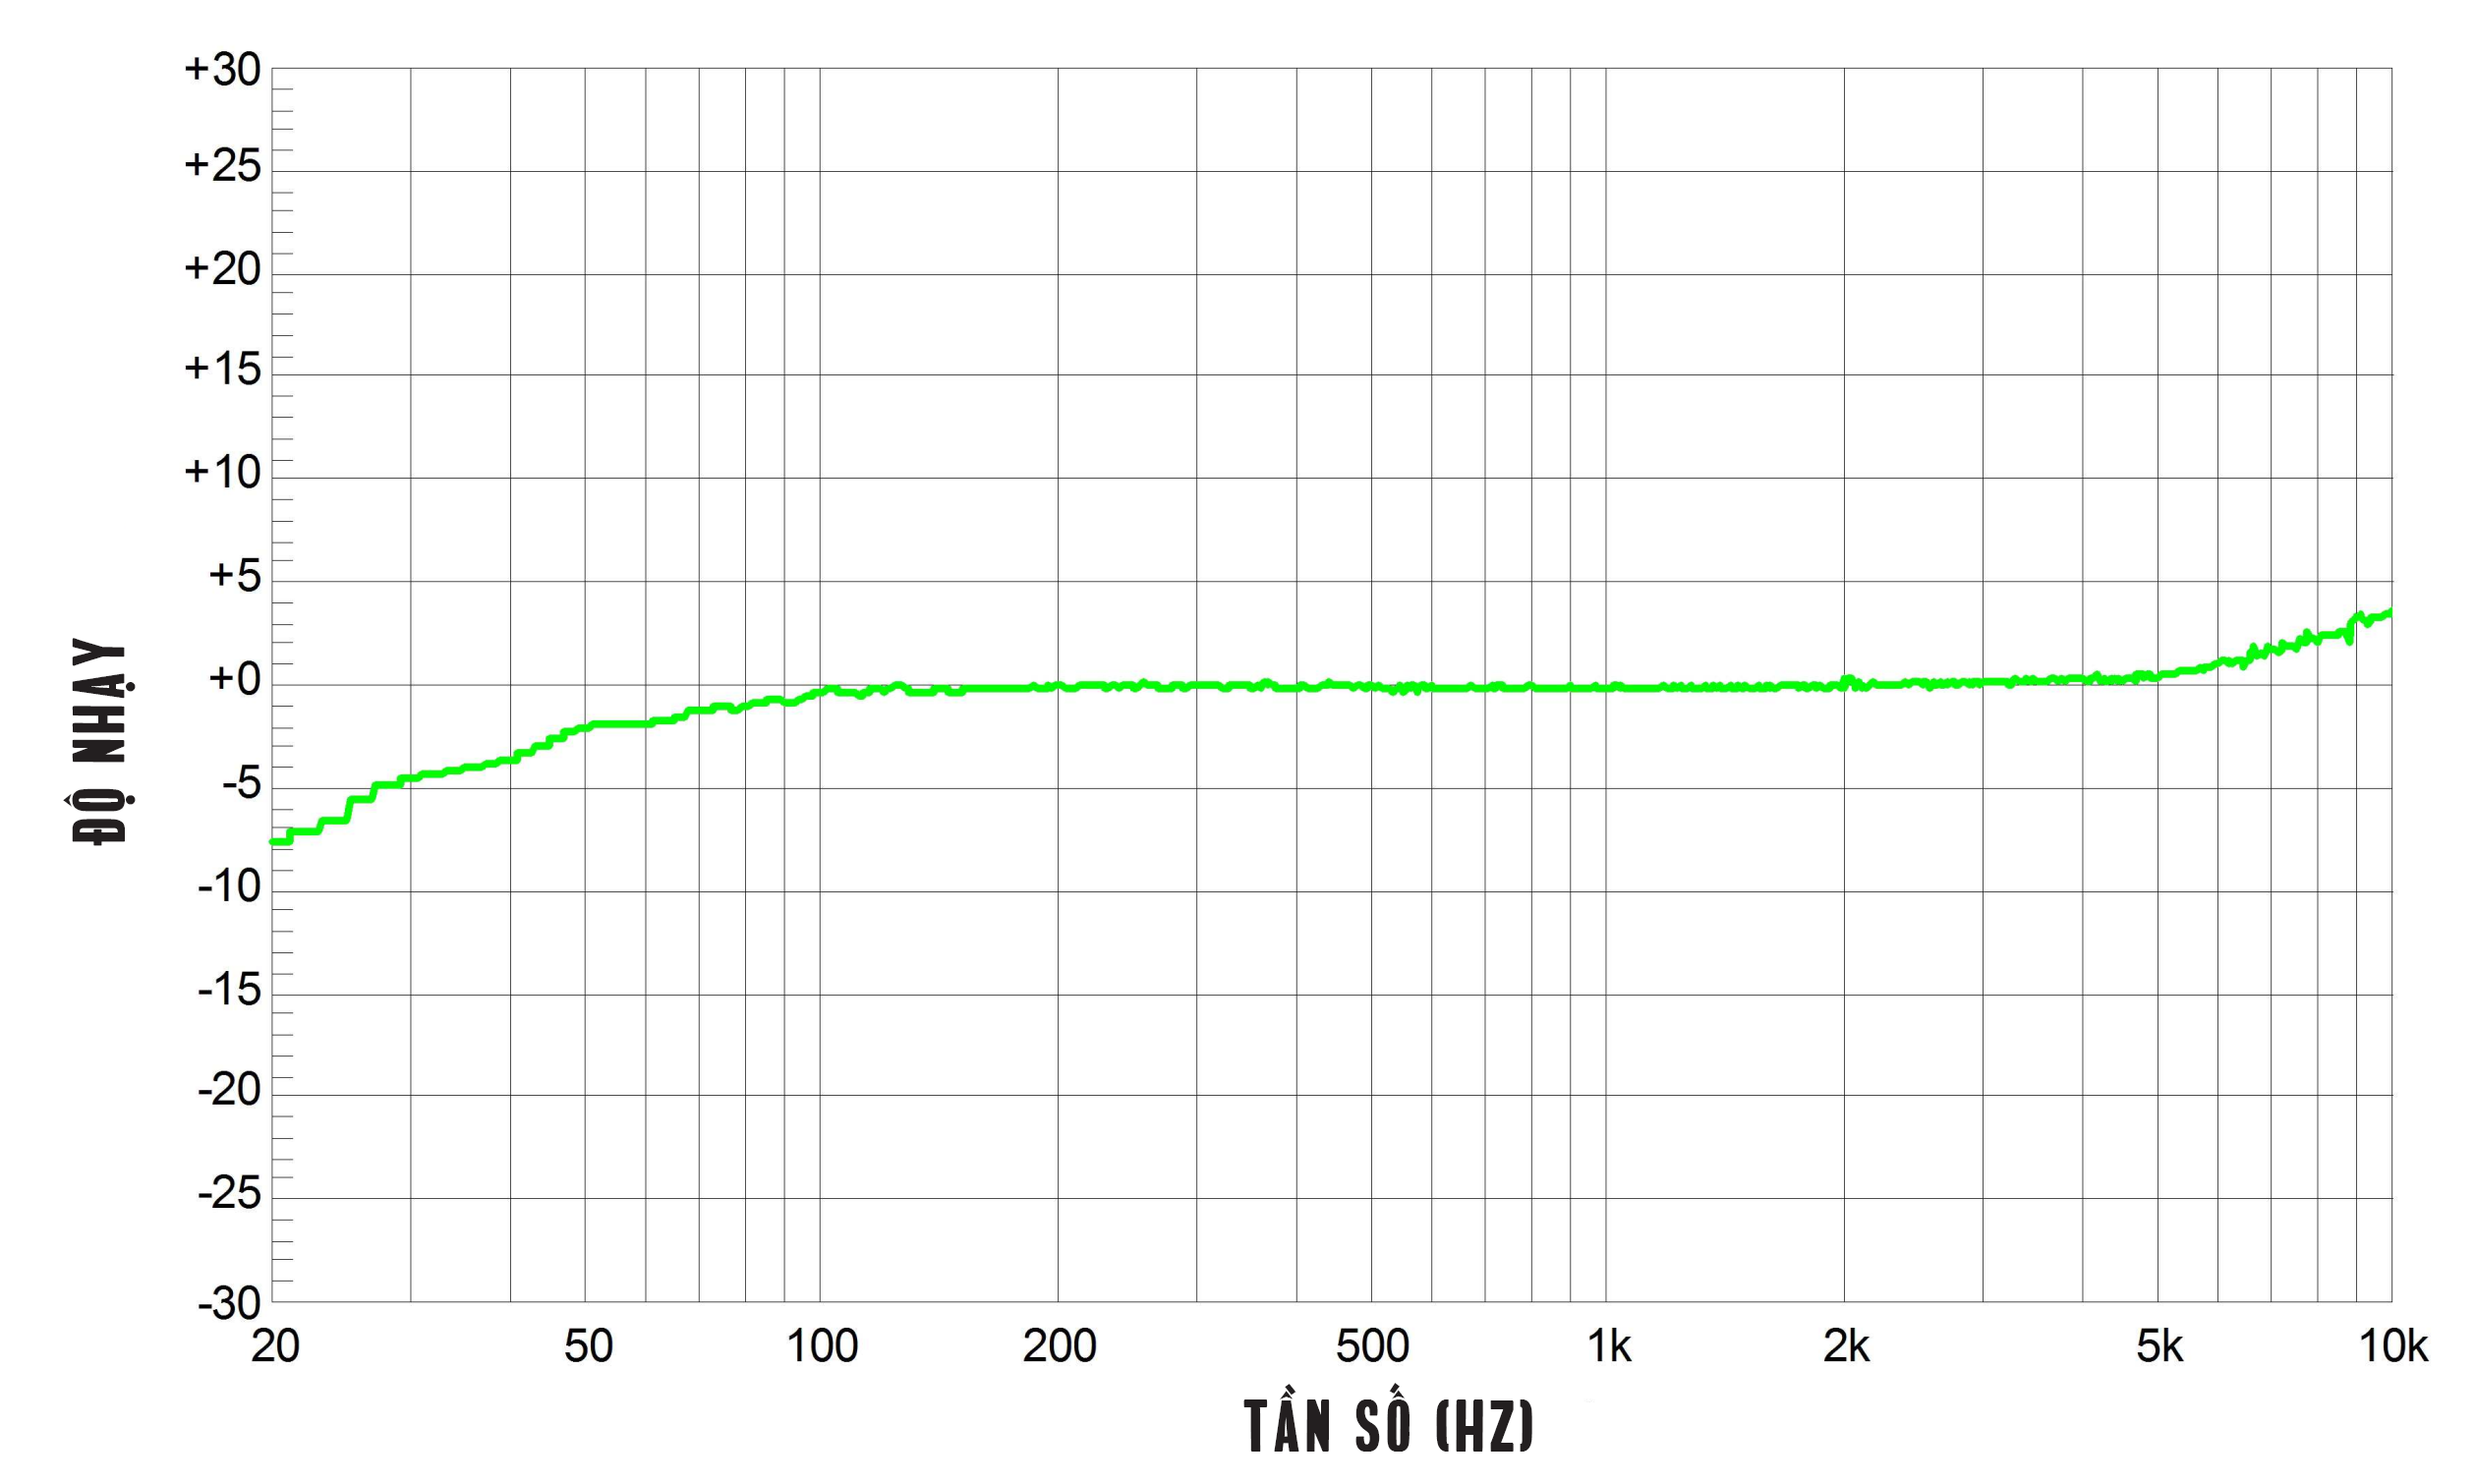
\includegraphics[width=13cm]{Images/Chuong2/do_nhay.png}
    \caption[Đáp ứng tần số của micro MP34DT01-M]{\bfseries \fontsize{12pt}{0pt}\selectfont Đáp ứng tần số của micro MP34DT01-M}
    \label{do_nhay}
\end{figure}

    \item Dải thông từ 0 đến 6kHz.\\
    Với việc âm thanh thu được chỉ ổn định trong tần số 100Hz đến 5kHz (hình \ref{do_nhay}), điểm chuyển tiếp ở vị trí 6kHz là một điểm phù hợp.
    \item Dải dừng bắt đầu ở 10kHz: vì ở trên tần số 10kHz, micro không có hành vi gì (hình \ref{do_nhay}).

\end{itemize}

Từ đó, chúng ta tóm tắt các yêu cầu thiết kế như bảng \ref{spec}.
\begin{table}[H]
    \centering
    \caption[Các yêu cầu thiết kế của hệ thống]{\bfseries\fontsize{12pt}{0pt}\selectfont Các yêu cầu thiết kế của hệ thống}
    \begin{tabular}{|l|c|c|}
        \hline
        \multicolumn{1}{|c|}{\textbf{Yêu cầu}}                                  & \textbf{Thông tin} & \textbf{Đơn vị} \\ \hline
        \begin{tabular}[c]{@{}l@{}}Tốc độ lấy mẫu đầu vào \\ (PDM)\end{tabular} & 2304               & kHz             \\ \hline
        \begin{tabular}[c]{@{}l@{}}Tốc độ lấy mẫu đầu ra\\ (PCM)\end{tabular}   & 48                 & kHz             \\ \hline
        Hệ số decimation                                                        & 48                 & lần             \\ \hline
        Dải thông                                                               & 0 - 6                & kHz             \\ \hline
        Dải dừng                                                                & 10                  & kHz             \\ \hline
        Độ gợn sóng dải thông         & 0.1                & dB              \\ \hline
        Độ suy hao của dài dừng                                                 & 89                 & dB              \\ \hline
    \end{tabular}
    \label{spec}
\end{table}


\subsection{Thiết kế bộ lọc sử dụng hàm "remez" của Numpy}

Ở trong đề tài này, chúng ta sẽ thiết kế bộ lọc "Equiripple FIR" bằng thuật toán \textbf{Parks-McClellan} \cite{rao2018digital}. Trong thư viện \textit{Numpy} đã có sẵn hàm chức năng \textit{remez} để thiết kế các bộ lọc theo thông số được đặt ra, việc triển khai sẽ sử dụng ngôn ngữ \textit{Python}.

Dưới đây là mô tả của hàm remez:
\begin{table}[H]
\begin{tabular}{|l|}
\hline
\begin{tabular}[c]{@{}l@{}} \texttt{
\fontsize{10pt}{0pt}\selectfont def remez (numtaps, bands, desired, weight=None, Hz=None, type='bandpass', maxiter=25, }\\      \hspace{1.6cm} \texttt{
\fontsize{10pt}{0pt}\selectfont grid\_density=16, fs=None)}\end{tabular} \\ \hline
\end{tabular}
\end{table}

\noindent Trong đó, chúng ta cần chú ý những tham số sau: 
\begin{itemize}
    \item numtaps: số lượng hệ số của bộ lọc số.
    \item bands: danh sách chứa các đoạn tần số cần chú ý của bộ lọc số (dải thông, dải dừng).
    \item desired: danh sách chứa các giá trị mục tiêu mà bộ lọc số cần đạt được tại các đoạn tần số được chỉ định với 1 là dải thông và 0 là dải dừng.
    \item weight (tùy chọn): danh sách trọng số tương ứng với các đoạn tần số được chỉ định.
\end{itemize}

Hàm sẽ trả về mảng chứa các đáp ứng xung của bộ lọc và các thông số như độ suy hao dải dừng và độ gợn sóng. Tuy nhiên, 2 thông số trên sẽ phụ thuộc vào số lượng "taps" (hiện tại đang được xác định bằng tay). Việc sử dụng nhiều "taps" sẽ giúp bộ lọc đạt được các thông số đặt ra hoàn hảo hơn và ngược lại. Tuy nhiên để triển khai lên phần cứng, chúng ta cần tối ưu bộ lọc làm sao cho số "taps" nhỏ nhất mà vẫn đảm bảo được các chi tiêu đã đề ra trước đó.

\noindent \textbf{Tìm số lượng taps tối ưu cho bộ lọc} \label{toiuu}

Lần lượt tăng N từ giá trị 1, sau đó đưa các tham số vào hàm \textbf{remez}, nó sẽ trả về độ suy hao của dải dừng và độ gợn sóng của dải thông. Lần lượt so sánh nó với yêu cầu đầu ra đã đặt ra. Đến khi hàm trả về kết quả lớn hơn hoặc bằng với yêu cầu thiết kế thì N ở vị trí này là số "taps" tối ưu nhất cho bộ lọc.
\begin{figure}[H]
    \centering
    \includesvg[width=14cm]{Images/Chuong3/MoDau/test_fir.svg}
    \caption[Biểu đồ của độ suy hao dải thông và độ gợn sóng ứng theo số lượng taps]{\bfseries \fontsize{12pt}{0pt}\selectfont Biểu đồ của độ suy hao dải thông và độ gợn sóng ứng theo số lượng taps}
    \label{tapsss}
\end{figure}

Hình \ref{tapsss} mô tả biểu đồ về suy hao dải dừng và độ gợn sóng ứng với số lượng taps ứng với trường hợp độ suy hao dải dừng 89 dB, độ gợn sóng 0.04 dB, dải dừng 10 - 24 kHz, dải thông 0 - 10 kHz. Chúng ta có thể thấy ở số lượng taps là 50 thì bộ lọc đáp ứng vừa đủ tất cả các yêu cầu.
\subsection{Thiết kế bộ chuyển đổi  PDM sang PCM}
Các thiết kế được đề xuất sẽ bám sát vào mô hình của bộ chuyển đổi đã trình bày ở mục \ref{mohinhpdm2pcm}.
\subsubsection{Ý tưởng thiết kế đơn giản} \label{dongian}
Không thực sự cần một kiến trúc bộ lọc phức tạp để chuyển đổi PDM sang PCM, chúng ta chỉ cần 1 bộ lọc thông thấp duy nhất là đã có thể đáp ứng được các thông số ở trên.

Bộ lọc thông thấp sẽ có các thông số như sau: 
\begin{itemize}
    \item Dải thông: 0 - 6 kHz
    \item Dải dừng: 10 kHz - 2304kHz
    \item Độ suy hao dải dừng: 89dB
    \item Độ gợn sóng của dải thông: 0.1dB
\end{itemize}

Sau tiến hành chạy thuật toán \textit{remez}, chúng ta có bộ lọc có 2116 taps,  biểu đồ đáp ứng tần số và đáp ứng xung mô tả lần lượt ở hình \ref{filter_the_damn_thing} và \ref{filter_the_damn_thing_impulse}.
\begin{figure}[H]
    \centering
    \includesvg[width=14cm]{Images/Chuong3/filter_the_damn_thing.svg}
    \caption[Đáp ứng tần số của bộ lọc đơn giản]{\bfseries \fontsize{12pt}{0pt}\selectfont Đáp ứng tần số của bộ lọc đơn giản}
    \label{filter_the_damn_thing}
\end{figure}
\begin{figure}[H]
    \centering
    \includesvg[width=14cm]{Images/Chuong3/filter_the_damn_thing_impulse.svg}
    \caption[Đáp ứng xung của bộ lọc đơn giản]{\bfseries \fontsize{12pt}{0pt}\selectfont Đáp ứng xung của bộ lọc đơn giản}
    \label{filter_the_damn_thing_impulse}
\end{figure}

Bộ trên có độ suy hao dải dừng là 89.035 dB, độ gợn sóng 0.01415 dB hoàn toàn thỏa mãn với yêu cầu thiết kế. Nhưng có một vấn đề, đó là số taps lớn dẫn đến phép nhân trong 1 giây khá lớn ($48000 \times 2216 = 106M \text{ phép}/s$). Trong thiết kế phần cứng, đồng nghĩa chúng ta phải dùng đến 2216 bộ nhân, điều đó gây nên hao phí tài nguyên nghiêm trọng.

\textbf{Kết luận}: việc sửa dụng một bộ lọc thông thấp duy nhất không được cho là khả thi gây hao phí tài nguyên phần cứng. Phần sau sẽ trình bày kiểu thiết kế sử dụng nhiều bộ lọc tối ưu và xử lý ở nhiều miền tần số.

\subsubsection{Thiết kế bộ chuyển đổi nhiều giai đoạn sử dụng hạ tần (Decimation)}
Có rất nhiều kiến trúc đường ống để khử tín hiệu mẫu ở tốc độ cao xuống thấp \cite{pipelie1} - \cite{pipelie2}, về cơ bản sẽ được rút gọn thành các khối như hình \ref{pipeline_top}:
\begin{itemize}
    \item Một bộ lọc CIC phía trước
    \item Một hoặc nhiều bộc lọc Half Band ở giữa
    \item Một bộ lọc FIR ở phía sau
\end{itemize}

\begin{figure}[H]
    \centering
    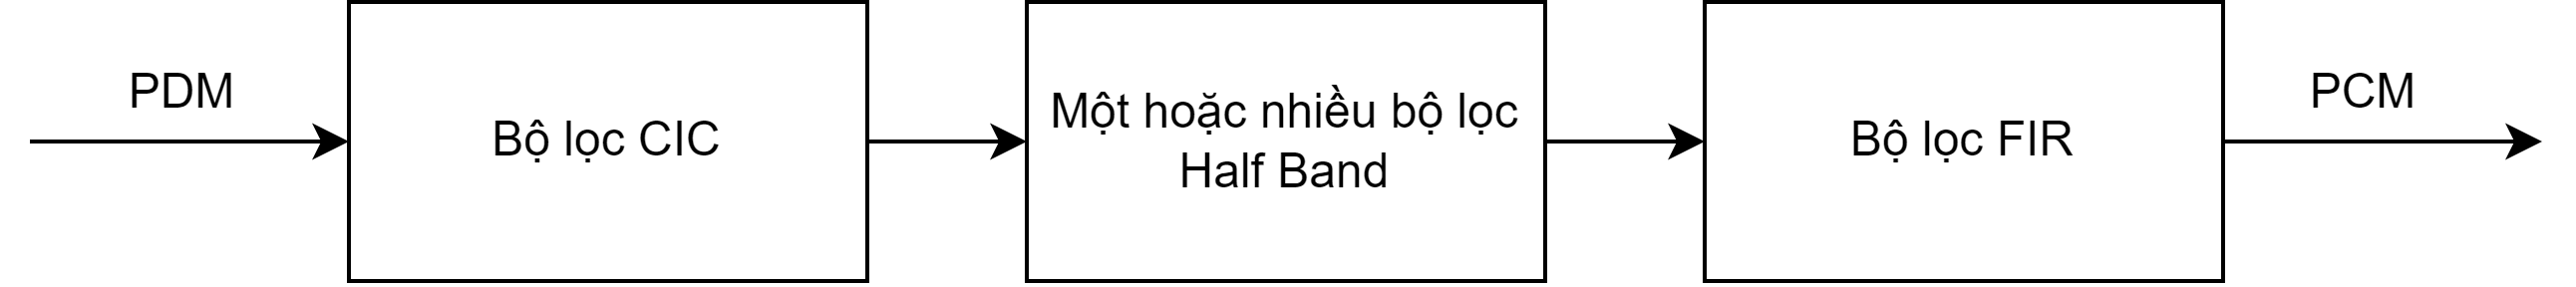
\includegraphics[width=15cm]{Images/Chuong3/pipeline_top.png}
    \caption[Sơ đồ khối của thiết kế dạng nhiều giai đoạn]{\bfseries \fontsize{12pt}{0pt}\selectfont Sơ đồ khối của thiết kế dạng nhiều giai đoạn}
    \label{pipeline_top}
\end{figure}
Lý do cho sự sắp xếp này là để phù hợp ràng buộc thiết kế như tốc độ xung nhịp và đặc biệt là mức sử dụng tài nguyên.
\begin{itemize}
    \item Bộ lọc CIC chỉ yêu cầu bộ cộng và bộ trễ chứ không yêu cầu bộ nhân. Điều này là cho thiết kế giảm đi một diện tích đáng kể.
    \item Việc không sử dụng bộ nhân cũng làm cho bộ lọc CIC dễ dàng chạy được ở tần số cao
    \item Bộ lọc hand Band chỉ yêu cầu khoảng 50\% phép nhân so với bộ lọc FIR tương đương.
    \item Việc sử dụng 2 bộ lọc CIC và Half Band vẫn chưa đủ điều kiện để lọc triệt để tín hiệu cần thu, dẫn đến việc phải sử dụng bộ FIR sau cùng. Nhưng bộ lọc này chạy ở tần số thấp và tài nguyên là không đáng kể.
\end{itemize}
\paragraph{Lựa chọn các tham số bộ lọc CIC}
Vì bộ lọc CIC không sử dụng bất kỳ bộ nhân nào, các thông số của bộ lọc chỉ phụ thuộc vào 2 tham số là số tầng và kích thước cửa số. Tuy nhiên, các bộ lọc CIC có độ gợn của dải thông trở nên ngày càng tồi tệ hơn với tần số tăng và số lượng các tầng tăng.

Do yêu cầu thiết kế có hệ số decimation là 48, do đó có 9 tỷ lệ có thể được chọn cho CIC: 2 3 4 6 8 12 16 24 48.

Hình \ref{cic_ratios_overview} mô tả đáp ứng tần số của bộ lọc CIC với tất cả các tỷ lệ decimation nói trên và 5 tầng. Gạch nối màu đỏ biểu thị ranh giới 6 kHz cần thu tín hiệu, chúng ta tiếp tục phân tích bằng cách phóng to (hình \ref{cic_ratios_zoom}). Dễ dành nhận ra ở dải tần 0 - 6 kHz và độ gợn sóng 0.1 dB, tỷ lệ Decimation từ 16 trở đi vi phạm yêu cầu thiết kế đặt ra. Điều đó có thể khắc phục bằng cách tăng số tầng của bộ lọc nhưng sẽ có một rắc rối đó là sẽ làm giảm độ suy hao của dải dừng.

\begin{figure}[H]
    \centering
    \includesvg[width=15cm]{Images/Chuong3/cic_ratios_overview.svg}
    \caption[Đáp ứng tần số của bộ lọc CIC 5 tầng với tất cả hệ số Decimation]{\bfseries \fontsize{12pt}{0pt}\selectfont Đáp ứng tần số của bộ lọc CIC 5 tầng với tất cả hệ số Decimation}
    \label{cic_ratios_overview}
\end{figure}

\begin{figure}[H]
    \centering
    \includesvg[width=15cm]{Images/Chuong3/cic_ratios_zoom.svg}
    \caption[Đáp ứng tần số của bộ lọc CIC 5 tầng với tất cả hệ số Decimation (phóng to)]{\bfseries \fontsize{12pt}{0pt}\selectfont Đáp ứng tần số của bộ lọc CIC 5 tầng với tất cả hệ số Decimation (phóng to)}
    \label{cic_ratios_zoom}
\end{figure}

Để đơn giản, chúng ta sẽ phải giới hạn tỷ lệ decimation và số lượng các tầng sao cho độ gợn dải thông không vượt quá một giá trị tối đa nhất định. Ở đây sẽ chọn độ gợn tối đa là 0.05 dB như vậy các bộ lọc phía sau phải đáp ứng được 0.05 dB còn lại (1 - 0.05 = 0.05 dB).

Để tìm ra thông số CIC thỏa mãn cả yêu cầu về dải thông và dải dừng, chúng ta sẽ tập trung vào bảng \ref{abc}. Nên chọn số tầng thấp nhất có thể để giảm được số lượng độ rộng của thanh ghi và các bộ cộng. Từ đó có thể đáp ứng được vấn đề về tài nguyên của hệ thống số.

 \noindent Quan sát bảng \ref{abc}, các \textbf{phương án} sau được đưa ra:
\begin{enumerate}
    \item \textbf{Tỷ lệ Decimation 6x và số tầng 3}: phương án này yêu cầu thêm 3 bộ lọc Half Band và 1 bộ lọc FIR cuối để đáp ứng được các thông số cuối cùng.
    \item \textbf{Tỷ lệ Decimation 8x và số tầng 4}: phương án này yêu cần cần thêm tỷ lệ Decimation phía sau là 6x, đồng nghĩa với dùng 1 bộ lọc Half Band và 1 bộ lọc FIR cuối kèm theo 1 bộ decimation 3x.
    \item \textbf{Tỷ lệ Decimation 12x và số tầng 4}: mặc dùng phương án này chưa đáp ứng được độ gợn sóng của dải thông (0.056 db, vượt 0.006 dB so với yêu cầu), nhưng chênh lệch này rất nhỏ. Với phương án này yêu cầu thêm 2 bộ lọc Half Band và 1 bộ lọc FIR. \label{choose}
\end{enumerate}

Các phương án có tỷ lệ Decimation từ 4 trở xuống hoàn toàn có thể đáp ứng được thiết kế. Tuy nhiên, việc chọn như thế sẽ gây nên hệ số decimation cho các bộ lọc phía sau lớn, đồng nghĩa với việc phải sử dụng nhiều bộ lọc Half Band gây tốn nhiều tài nguyên. Trái với phương châm của thiết kế là sử dụng bộ CIC với thông số tối ưu nhất để các bộ lọc sau đơn giản nhất có thể.

\vspace{2cm}
\begin{table}[H]
    \centering
    \caption[Độ gợn sóng và độ suy hao của dải dừng của bộ lọc CIC ở nhiều cấu hình khác nhau (dB)]{\bfseries\fontsize{12pt}{0pt}\selectfont Độ gợn sóng và độ suy hao của dải dừng của bộ lọc CIC ở nhiều cấu hình khác nhau (dB)}
\begin{tabular}{|c|l|l|l|l|l|l|}
\hline
\backslashbox{\textbf{Tỷ lệ}}{\textbf{Tầng}} &
  \multicolumn{1}{c|}{\textbf{1}} &
  \multicolumn{1}{c|}{\textbf{2}} &
  \multicolumn{1}{c|}{\textbf{3}} &
  \multicolumn{1}{c|}{\textbf{4}} &
  \multicolumn{1}{c|}{\textbf{5}} &
  \multicolumn{1}{c|}{\textbf{6}} \\ \hline
\textbf{2} &
  \begin{tabular}[c]{@{}l@{}}-0,0003\\ -37,3\end{tabular} &
  \begin{tabular}[c]{@{}l@{}}-0,0006\\ -74,6\end{tabular} &
  \begin{tabular}[c]{@{}l@{}}-0,0009\\ -112,0\end{tabular} &
  \begin{tabular}[c]{@{}l@{}}-0,0012\\ -149,3\end{tabular} &
  \begin{tabular}[c]{@{}l@{}}-0,0015\\ -186,6\end{tabular} &
  \begin{tabular}[c]{@{}l@{}}-0,0018\\ -223,9\end{tabular} \\ \hline
\textbf{3} &
  \begin{tabular}[c]{@{}l@{}}-0,0008\\ -36,0\end{tabular} &
  \begin{tabular}[c]{@{}l@{}}-0,0016\\ -72,0\end{tabular} &
  \begin{tabular}[c]{@{}l@{}}-0,0024\\ -108,0\end{tabular} &
  \begin{tabular}[c]{@{}l@{}}-0,0032\\ -144,0\end{tabular} &
  \begin{tabular}[c]{@{}l@{}}-0,0039\\ -180,0\end{tabular} &
  \begin{tabular}[c]{@{}l@{}}-0,0047\\ -216,0\end{tabular} \\ \hline
\textbf{4} &
  \begin{tabular}[c]{@{}l@{}}-0,0015\\ -34,2\end{tabular} &
  \begin{tabular}[c]{@{}l@{}}-0,0030\\ -68,4\end{tabular} &
  \begin{tabular}[c]{@{}l@{}}-0,0044\\ -102,6\end{tabular} &
  \begin{tabular}[c]{@{}l@{}}-0,0059\\ -136,8\end{tabular} &
  \begin{tabular}[c]{@{}l@{}}-0,0074\\ -171,0\end{tabular} &
  \begin{tabular}[c]{@{}l@{}}-0,0089\\ -205,2\end{tabular} \\ \hline
\textbf{6} &
  \begin{tabular}[c]{@{}l@{}}-0,0034\\ -31,1\end{tabular} &
  \begin{tabular}[c]{@{}l@{}}-0,0069\\ -62,2\end{tabular} &
  \begin{tabular}[c]{@{}l@{}}-0,0103\\ -93,3\end{tabular} &
  \begin{tabular}[c]{@{}l@{}}-0,0138\\ -124,4\end{tabular} &
  \begin{tabular}[c]{@{}l@{}}-0,0172\\ -155,5\end{tabular} &
  \begin{tabular}[c]{@{}l@{}}-0,0207\\ -186,6\end{tabular} \\ \hline
\textbf{8} &
  \begin{tabular}[c]{@{}l@{}}-0,0062\\ -28,7\end{tabular} &
  \begin{tabular}[c]{@{}l@{}}-0,0124\\ -57,4\end{tabular} &
  \begin{tabular}[c]{@{}l@{}}-0,0186\\ -86,1\end{tabular} &
  \begin{tabular}[c]{@{}l@{}}-0,0248\\ -114,8\end{tabular} &
  \begin{tabular}[c]{@{}l@{}}-0,0310\\ -143,5\end{tabular} &
  \begin{tabular}[c]{@{}l@{}}-0,0372\\ -172,2\end{tabular} \\ \hline
\textbf{12} &
  \begin{tabular}[c]{@{}l@{}}-0,0141\\ -25,2\end{tabular} &
  \begin{tabular}[c]{@{}l@{}}-0,0282\\ -50,3\end{tabular} &
  \begin{tabular}[c]{@{}l@{}}-0,0423\\ -75,5\end{tabular} &
  \begin{tabular}[c]{@{}l@{}}-0,0564\\ -100,6\end{tabular} &
  \begin{tabular}[c]{@{}l@{}}-0,0705\\ -125,8\end{tabular} &
  \begin{tabular}[c]{@{}l@{}}-0,0846\\ -150,9\end{tabular} \\ \hline
\textbf{16} &
  \begin{tabular}[c]{@{}l@{}}-0,0251\\ -22,6\end{tabular} &
  \begin{tabular}[c]{@{}l@{}}-0,0502\\ -45,2\end{tabular} &
  \begin{tabular}[c]{@{}l@{}}-0,0753\\ -67,7\end{tabular} &
  \begin{tabular}[c]{@{}l@{}}-0.1004\\ -90.3\end{tabular} &
  \begin{tabular}[c]{@{}l@{}}-0,1256\\ -112,9\end{tabular} &
  \begin{tabular}[c]{@{}l@{}}-0,1507\\ -135,5\end{tabular} \\ \hline
\textbf{24} &
  \begin{tabular}[c]{@{}l@{}}-0,0568\\ -18,8\end{tabular} &
  \begin{tabular}[c]{@{}l@{}}-0,1135\\ -37,7\end{tabular} &
  \begin{tabular}[c]{@{}l@{}}-0,1703\\ -56,5\end{tabular} &
  \begin{tabular}[c]{@{}l@{}}-0,2271\\ -75,3\end{tabular} &
  \begin{tabular}[c]{@{}l@{}}-0,2839\\ -94,2\end{tabular} &
  \begin{tabular}[c]{@{}l@{}}-0,3406\\ -113,0\end{tabular} \\ \hline
\textbf{48} &
  \begin{tabular}[c]{@{}l@{}}-0,2190\\ -12,2\end{tabular} &
  \begin{tabular}[c]{@{}l@{}}-0,4381\\ -24,4\end{tabular} &
  \begin{tabular}[c]{@{}l@{}}-0,6571\\ -36,6\end{tabular} &
  \begin{tabular}[c]{@{}l@{}}-0,8761\\ -48,8\end{tabular} &
  \begin{tabular}[c]{@{}l@{}}-1,0952\\ -61,0\end{tabular} &
  \begin{tabular}[c]{@{}l@{}}-1.3142\\ -73.2\end{tabular} \\ \hline
\end{tabular}
\label{abc}
\end{table}

\begin{table}[H]
    \centering
    \caption[Bảng tính toán tổng các phép nhân của từng phương án]{\bfseries\fontsize{12pt}{0pt}\selectfont Bảng tính toán tổng các phép nhân của từng phương án}
\begin{tabular}{|c|l|l|l|l|l|}
\hline
\textbf{Phương án} &
  \multicolumn{1}{c|}{\textbf{\begin{tabular}[c]{@{}c@{}}HB1\\ (phép/s)\end{tabular}}} &
  \multicolumn{1}{c|}{\textbf{\begin{tabular}[c]{@{}c@{}}HB2\\ (phép/s)\end{tabular}}} &
  \multicolumn{1}{c|}{\textbf{\begin{tabular}[c]{@{}c@{}}HB3\\ (phép/s)\end{tabular}}} &
  \multicolumn{1}{c|}{\textbf{\begin{tabular}[c]{@{}c@{}}FIR\\ (phép/s)\end{tabular}}} &
  \multicolumn{1}{c|}{\textbf{\begin{tabular}[c]{@{}c@{}}Tổng\\ (phép/s)\end{tabular}}} \\ \hline
\textbf{Phương án 1} &
  \begin{tabular}[c]{@{}l@{}}4 x 192 k\\ =768 k\end{tabular} &
  \begin{tabular}[c]{@{}l@{}}6 x 96 k\\ = 576 k\end{tabular} &
  \begin{tabular}[c]{@{}l@{}}10 x 48 k\\ = 480 k\end{tabular} &
  \begin{tabular}[c]{@{}l@{}}47 x 48 k\\ = 2256 k\end{tabular} &
  4080 k \\ \hline
\textbf{Phương án 2} &
  \begin{tabular}[c]{@{}l@{}}6 x 144 k\\ = 864 k\end{tabular} &
   &
   &
  \begin{tabular}[c]{@{}l@{}}141 x 48 k\\ = 6768 k\end{tabular} &
  4320 k \\ \hline
\textbf{Phương án 3} &
  \begin{tabular}[c]{@{}l@{}}6 x 96 k\\ = 576 k\end{tabular} &
  \begin{tabular}[c]{@{}l@{}}10 * 48 k \\ = 480 k\end{tabular} &
   &
  \begin{tabular}[c]{@{}l@{}}51 x 48 k\\ = 2448 k\end{tabular} &
  3504 k \\ \hline
\end{tabular}
\label{phepnhan}
\end{table}
Khi các thuộc tính của bộ lọc CIC đã được quyết định, thiết kế bộ lọc Half Band và FIR sẽ được chạy thuật toán Parks-McClellan/Remez và tối ưu (mục \ref{toiuu}) để đưa ra các hệ số bộ lọc chính xác. Từ đó, chúng ta có thể đưa ra số phép nhân xảy ra trong 1 giây, mô tả như bảng \ref{phepnhan}. Dễ dàng nhận ra \textbf{phương án 3} là phương án tối ưu nhất.

Giờ thì chúng ta có thể thấy rõ sự khác biệt giữa 2 kiến trúc đơn giản (mục \ref{dongian}) và sử dụng nhiều bộ lọc trên nhiều miền tần số khác nhau. Với 3504k phép nhân trên 1 giây so với 106M phép nhân trong 1 giây, nó được cải thiện hơn 30 lần.
\paragraph{Thiết kế bộ lọc Half Band và FIR} \label{design_fir}
Với phương án \hyperref[choose]{đã được chọn ở trên} (CIC 4 tầng, tỷ lệ Decimation 12x) thì hệ số Decimation chỉ còn lại là 4, điều đó đồng nghĩ với việc chúng ta chỉ cần sử dụng thêm 2 bộ lọc Half Band với tỷ lệ Decimation mỗi bộ lọc là 2 và một bộ lọc FIR ở tầng cuối cùng. 

Chúng ta có sơ đồ khối tổng quát của thiết kế như hình \ref{pipeline_new}.
\begin{figure}[H]
    \centering
    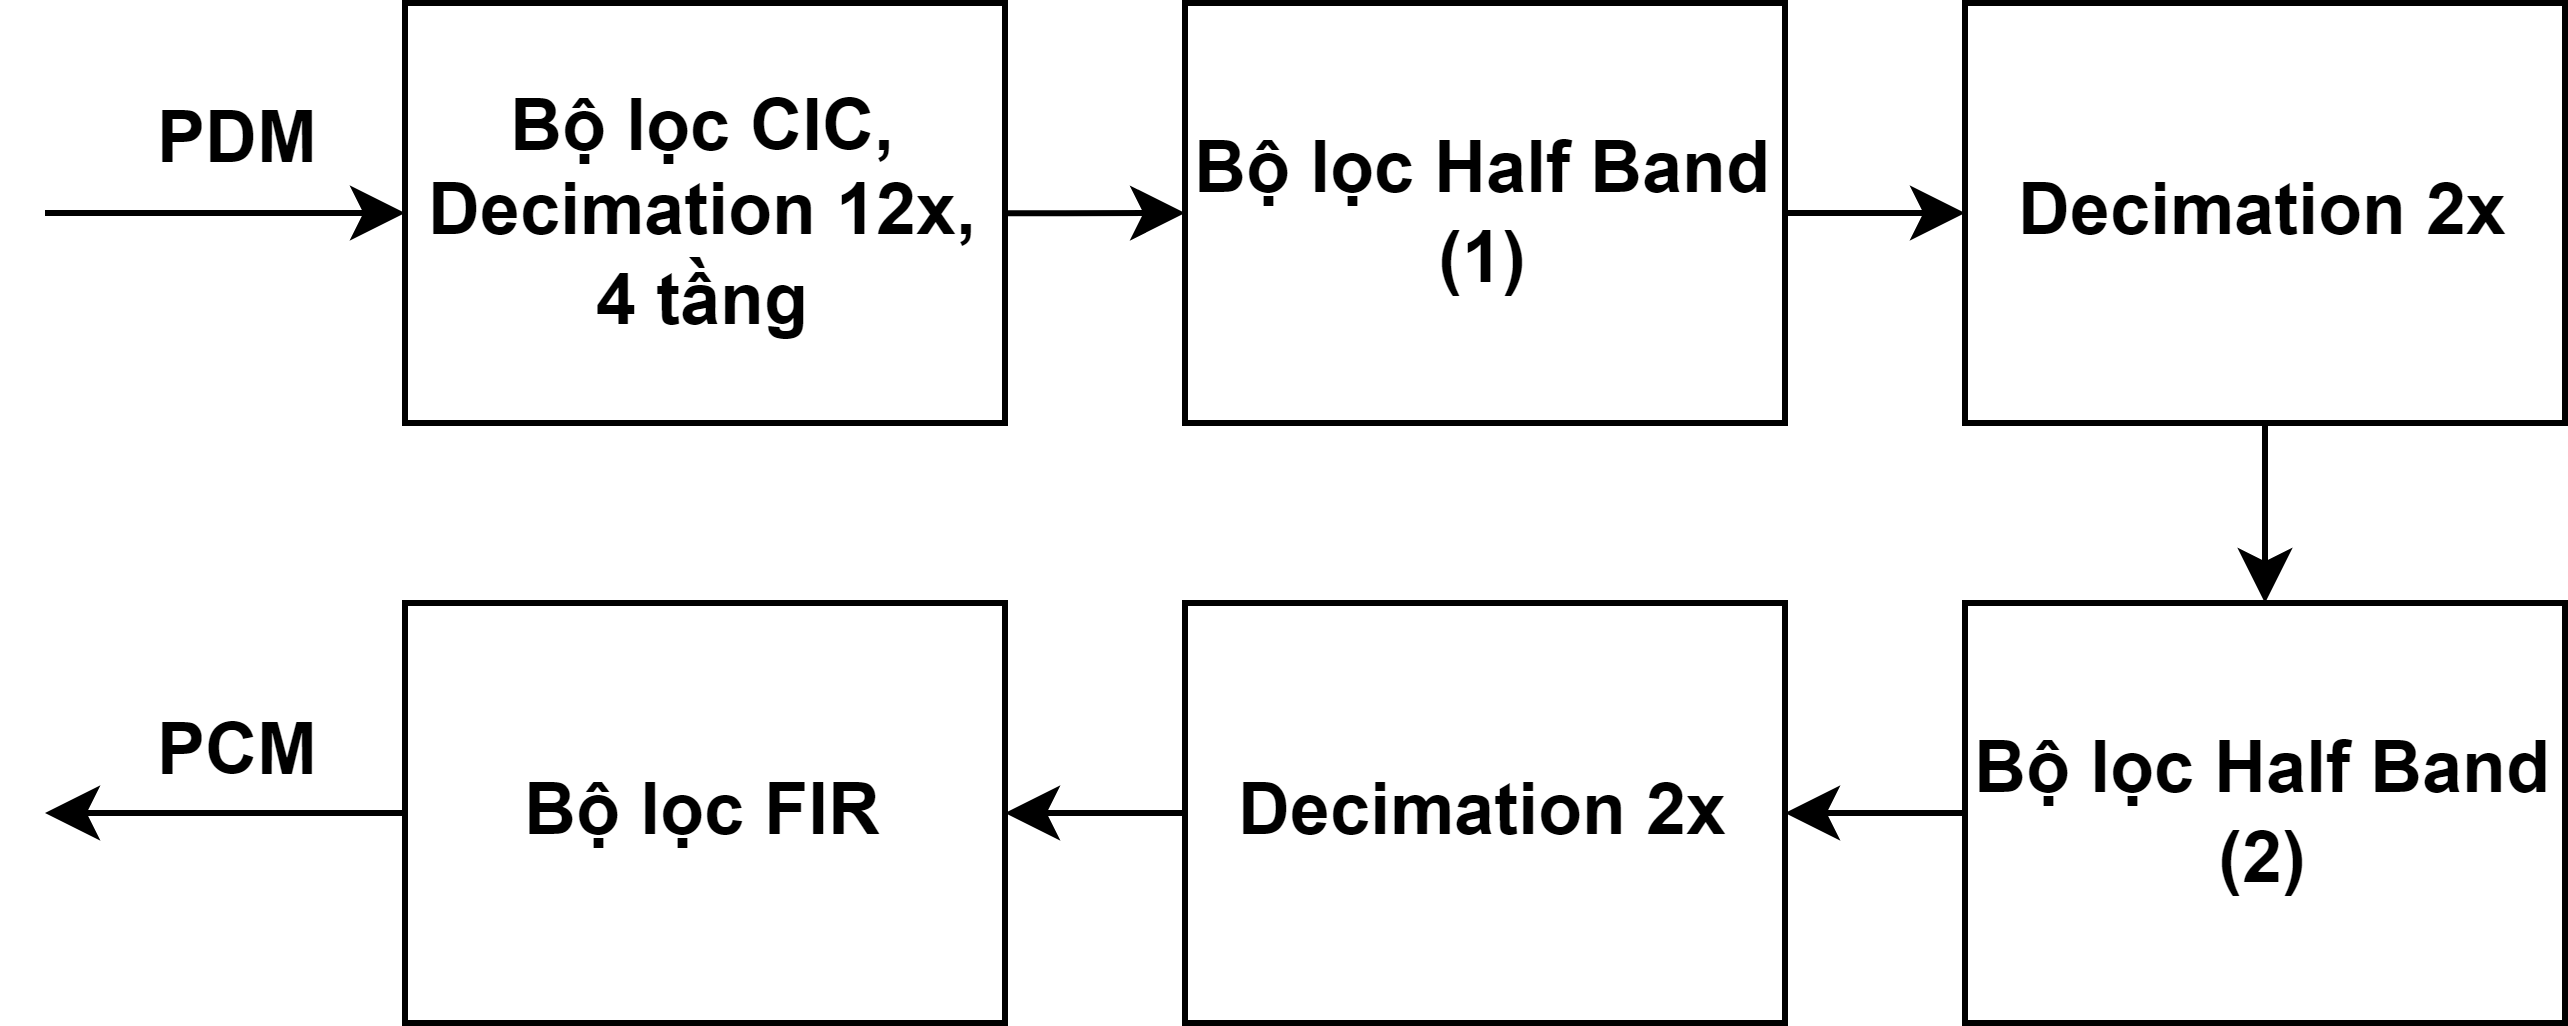
\includegraphics[width=11cm]{Images/Chuong3/pipeline_new_top.png}
    \caption[Sơ đồ khối tổng quát của bộ chuyển đổi nhiều giai đoạn]{\bfseries \fontsize{12pt}{0pt}\selectfont Sơ đồ khối tổng quát của bộ chuyển đổi nhiều giai đoạn}
    \label{pipeline_new}
\end{figure}
 \noindent Các bộ lọc sẽ phải đạt các thông số thiết kế tối thiểu như sau:
\begin{enumerate}
    \item \textbf{Bộ lọc CIC}: \\
    Hệ số Decimation: 12\\
    Số tầng: 4\\
    Độ gợn sóng của dải thông: $A_{CIC} =$ 0.0564 dB\\
    Tần số lấy mẫu: 2304 kHz
    \item \textbf{Bộ lọc Half Band (1)}:\\
    Tần số lấy mẫu: 192 kHz\\
    Dải thông: 0 - 10 kHz\\
    Điểm dừng: 86 kHz\\
    Độ gợn sóng của dải thông: $A_{HB1} = 0.1 - A_{CIC}$\\
    Độ suy hao của dải dừng: 89 dB
    \item \textbf{Bộ lọc Half Band (2)}:\\
    Tần số lấy mẫu: 96 kHz\\
    Dải thông: 0 - 10 kHz\\
    Điểm dừng: 38 kHz\\
    Độ gợn sóng của dải thông: $A_{HB2} = 0.1 - A_{CIC} - A_{HB1}$\\
    Độ suy hao của dải dừng: 89 dB
    \item \textbf{Bộ lọc FIR}:\\
    Tần số lấy mẫu: 48 kHz\\
    Dải thông: 0 - 6 kHz\\
    Điểm dừng: 10 kHz\\
    Độ gợn sóng của dải thông: $A_{HB2} = 0.1 - A_{CIC} - A_{HB1} - A_{HB2}$\\
    Độ suy hao của dải dừng: 89 dB
\end{enumerate}

 Phổ của từng giai đoạn mô tả như hình 
 \ref{t1}, \ref{t2}, \ref{t3}, \ref{t4} với phần màu xanh là phần tín hiệu cần lấy và phần màu vàng là phần tần số nhiễu phải được loại bỏ.
 \vspace{1.5cm}
 \begin{figure}[H]
    \centering
    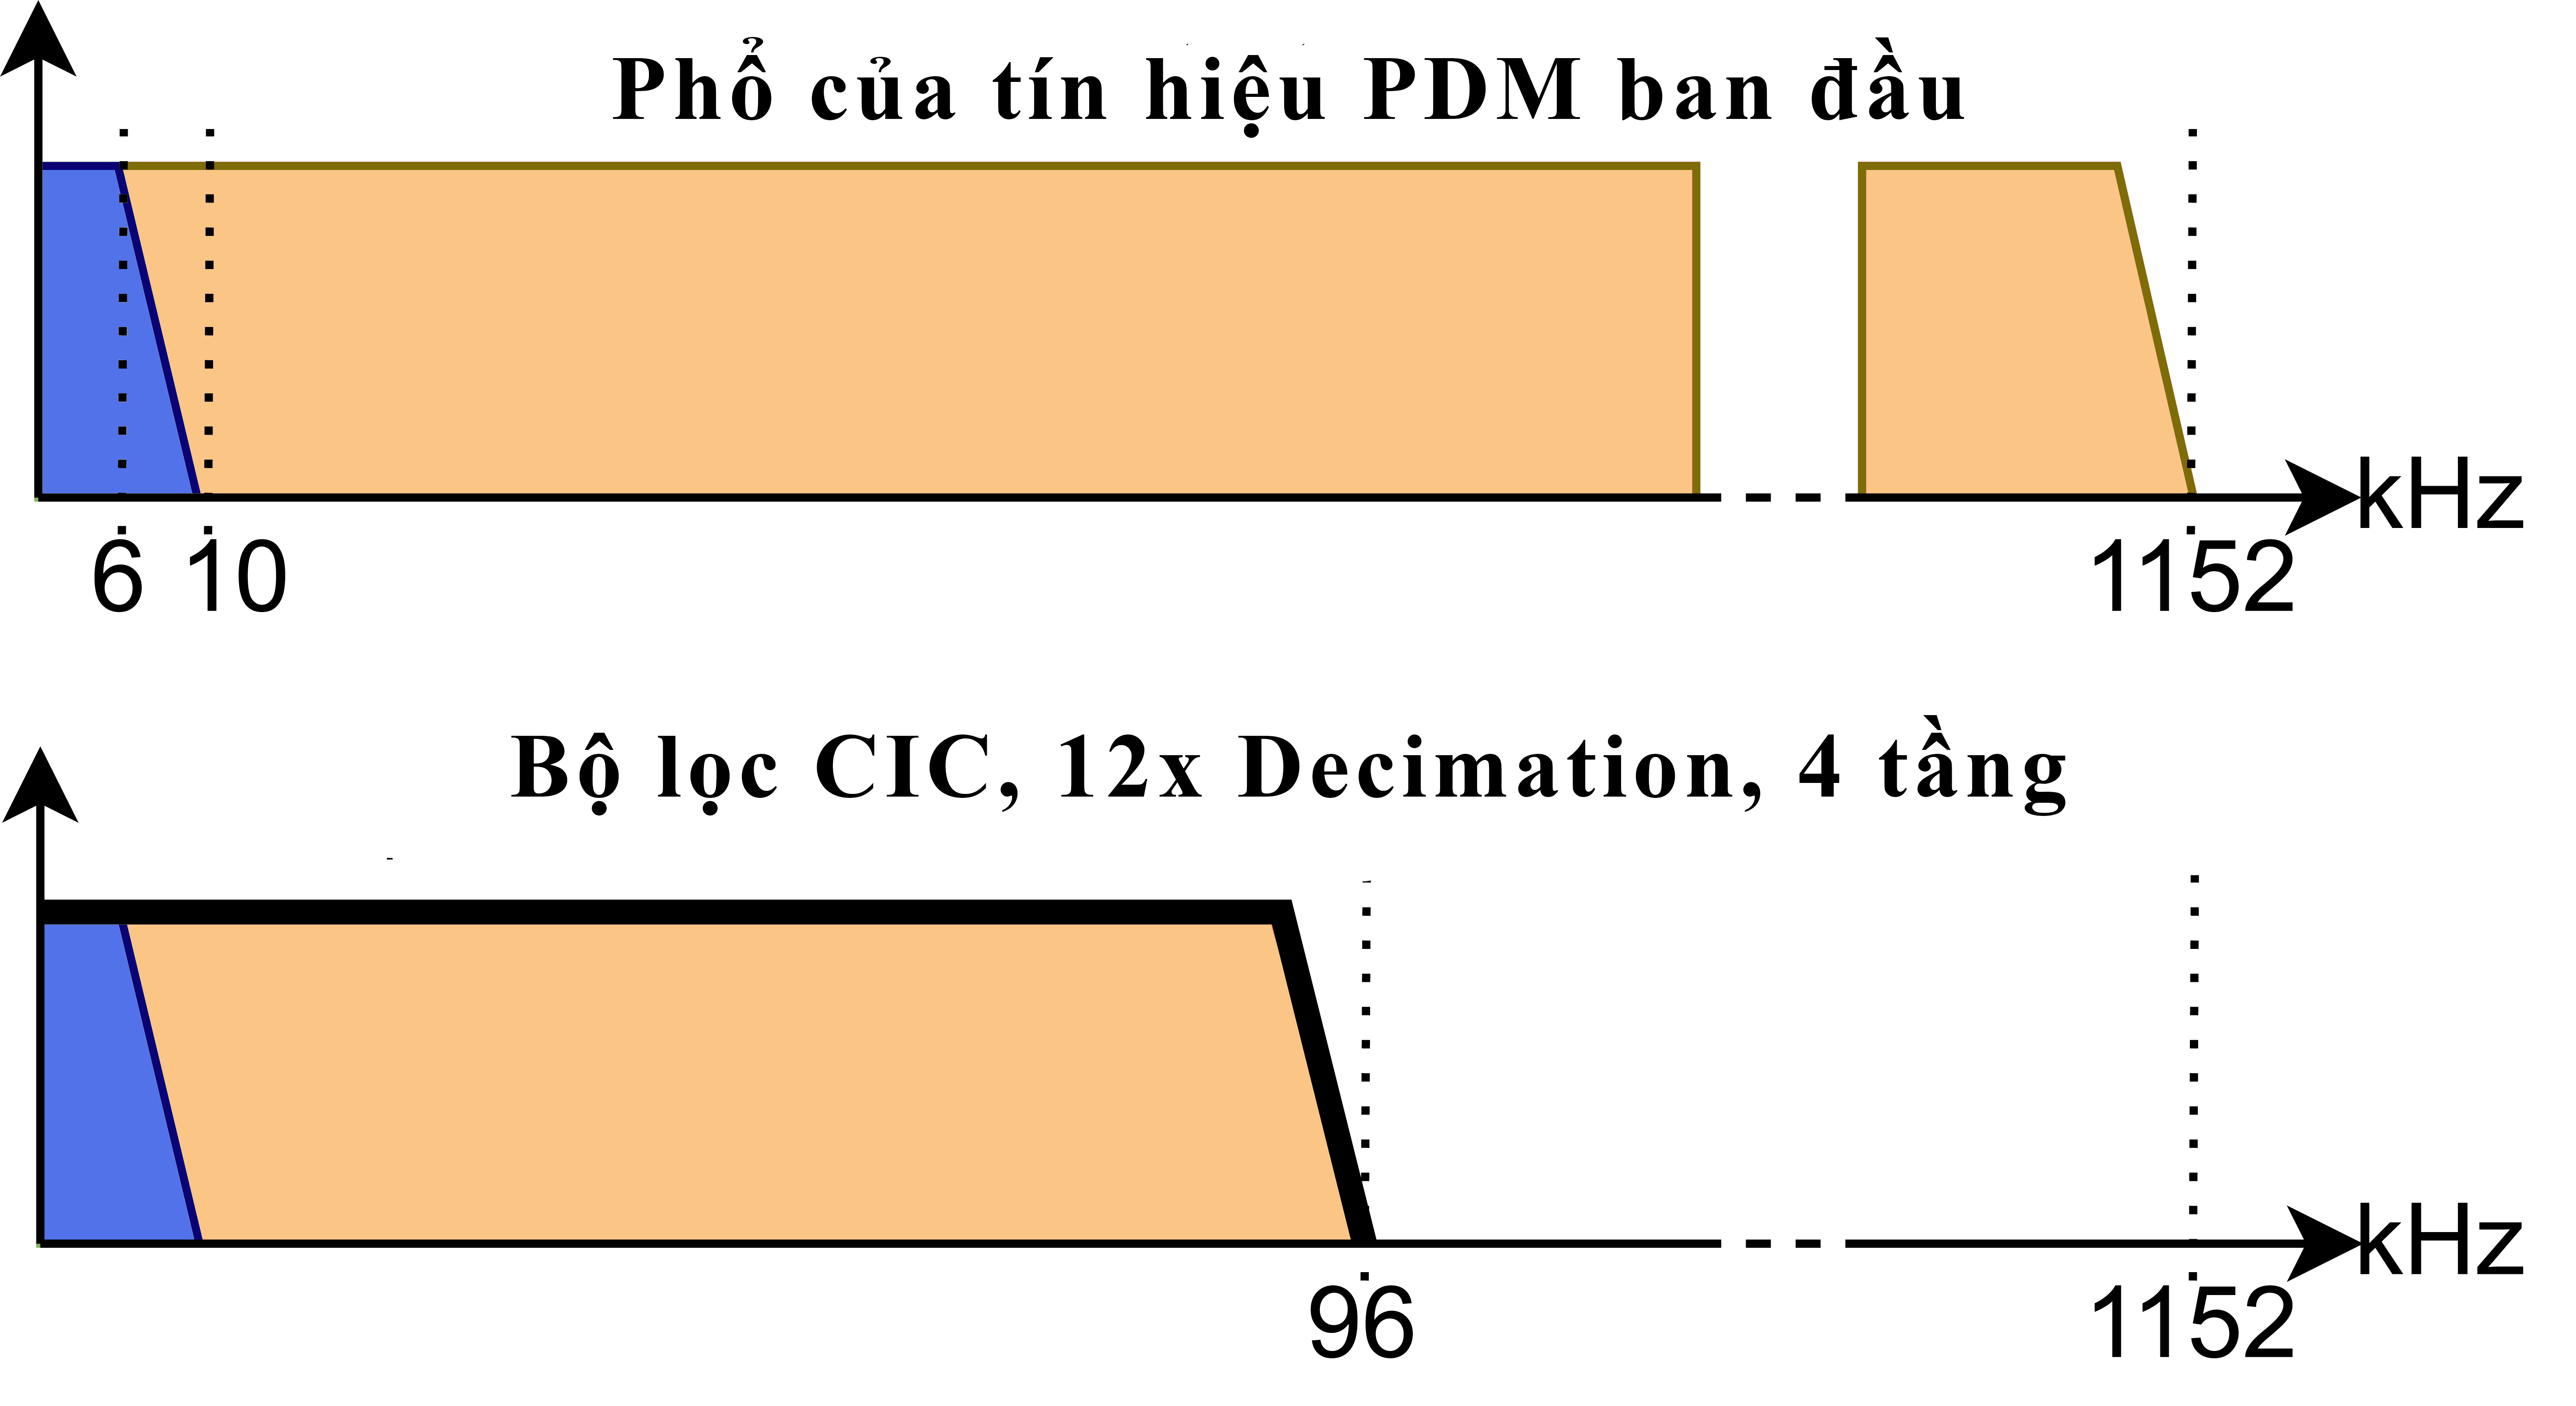
\includegraphics[width=11cm]{Images/Chuong3/1.png}
    \caption[Phổ của tín hiệu sau khi qua bộ lọc CIC]{\bfseries \fontsize{12pt}{0pt}\selectfont Phổ của tín hiệu sau khi qua bộ lọc CIC}
    \label{t1}
\end{figure}
\begin{figure}[H]
    \centering
    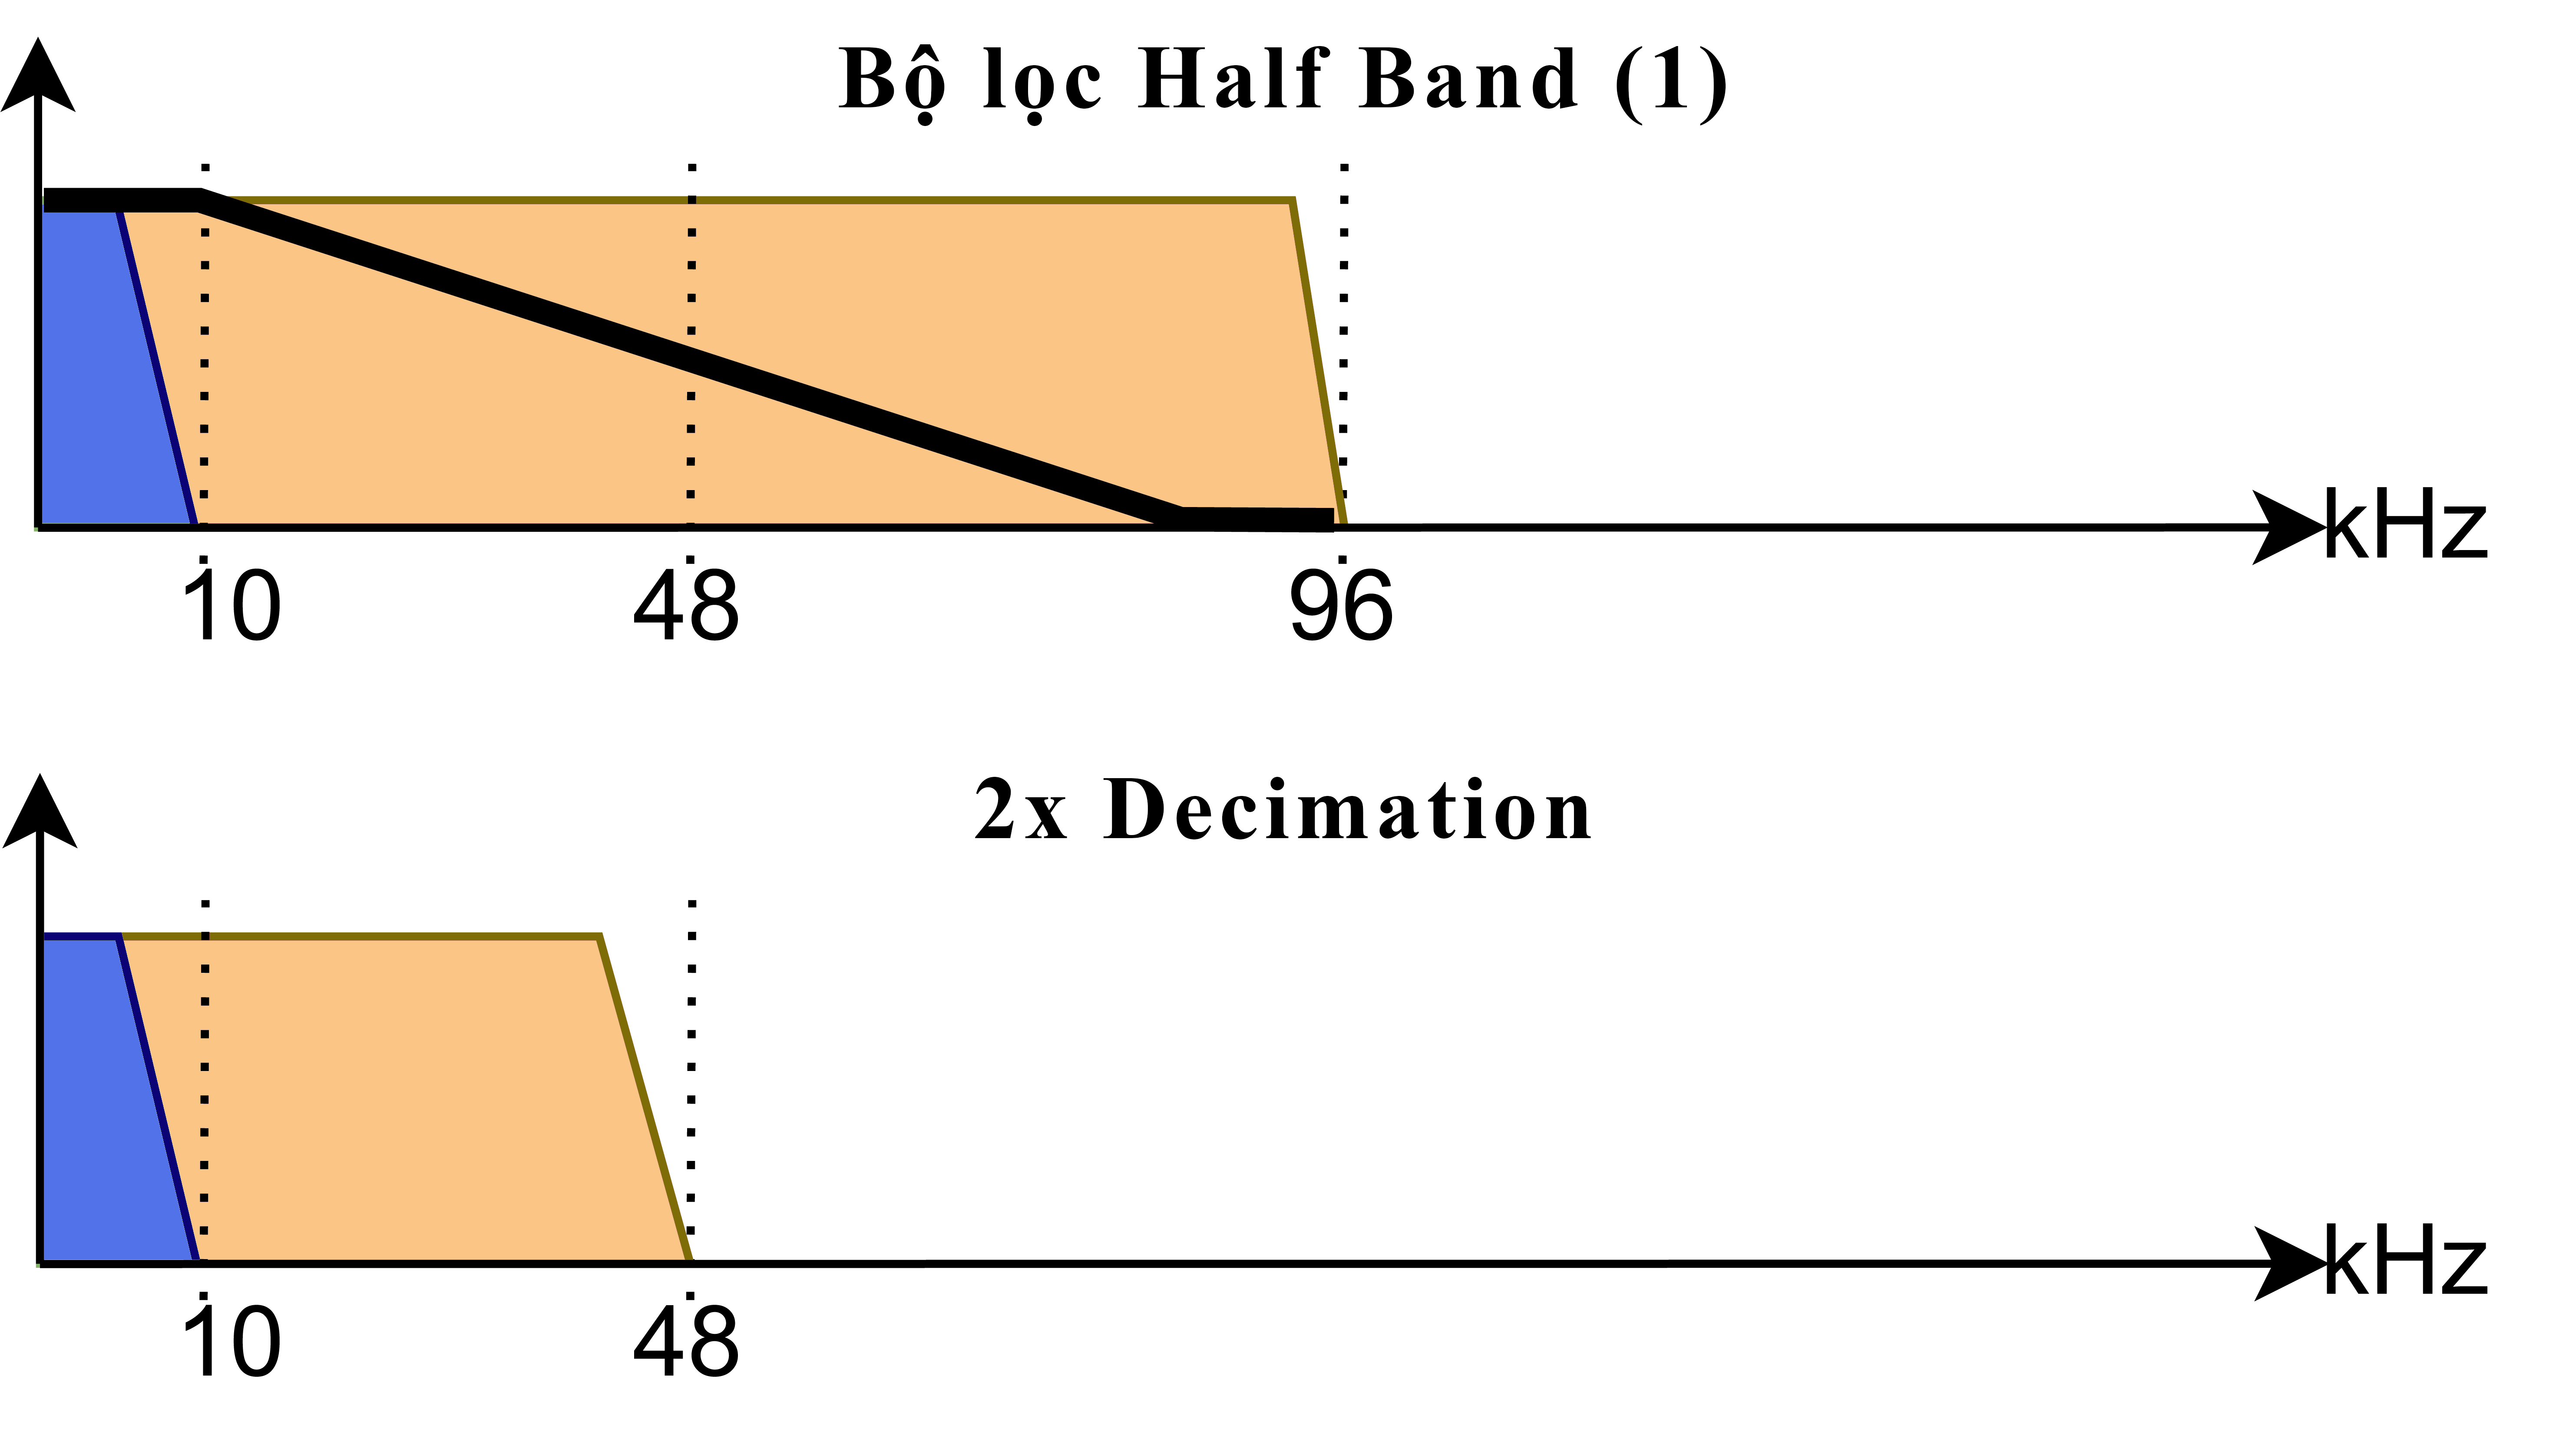
\includegraphics[width=11cm]{Images/Chuong3/2.png}
    \caption[Phổ của tín hiệu sau khi qua bộ lọc Half Band (1) và bộ Decimation 2x]{\bfseries \fontsize{12pt}{0pt}\selectfont Phổ của tín hiệu sau khi qua bộ lọc Half Band (1) và bộ Decimation 2x}
    \label{t2}
\end{figure}
\begin{figure}[H]
    \centering
    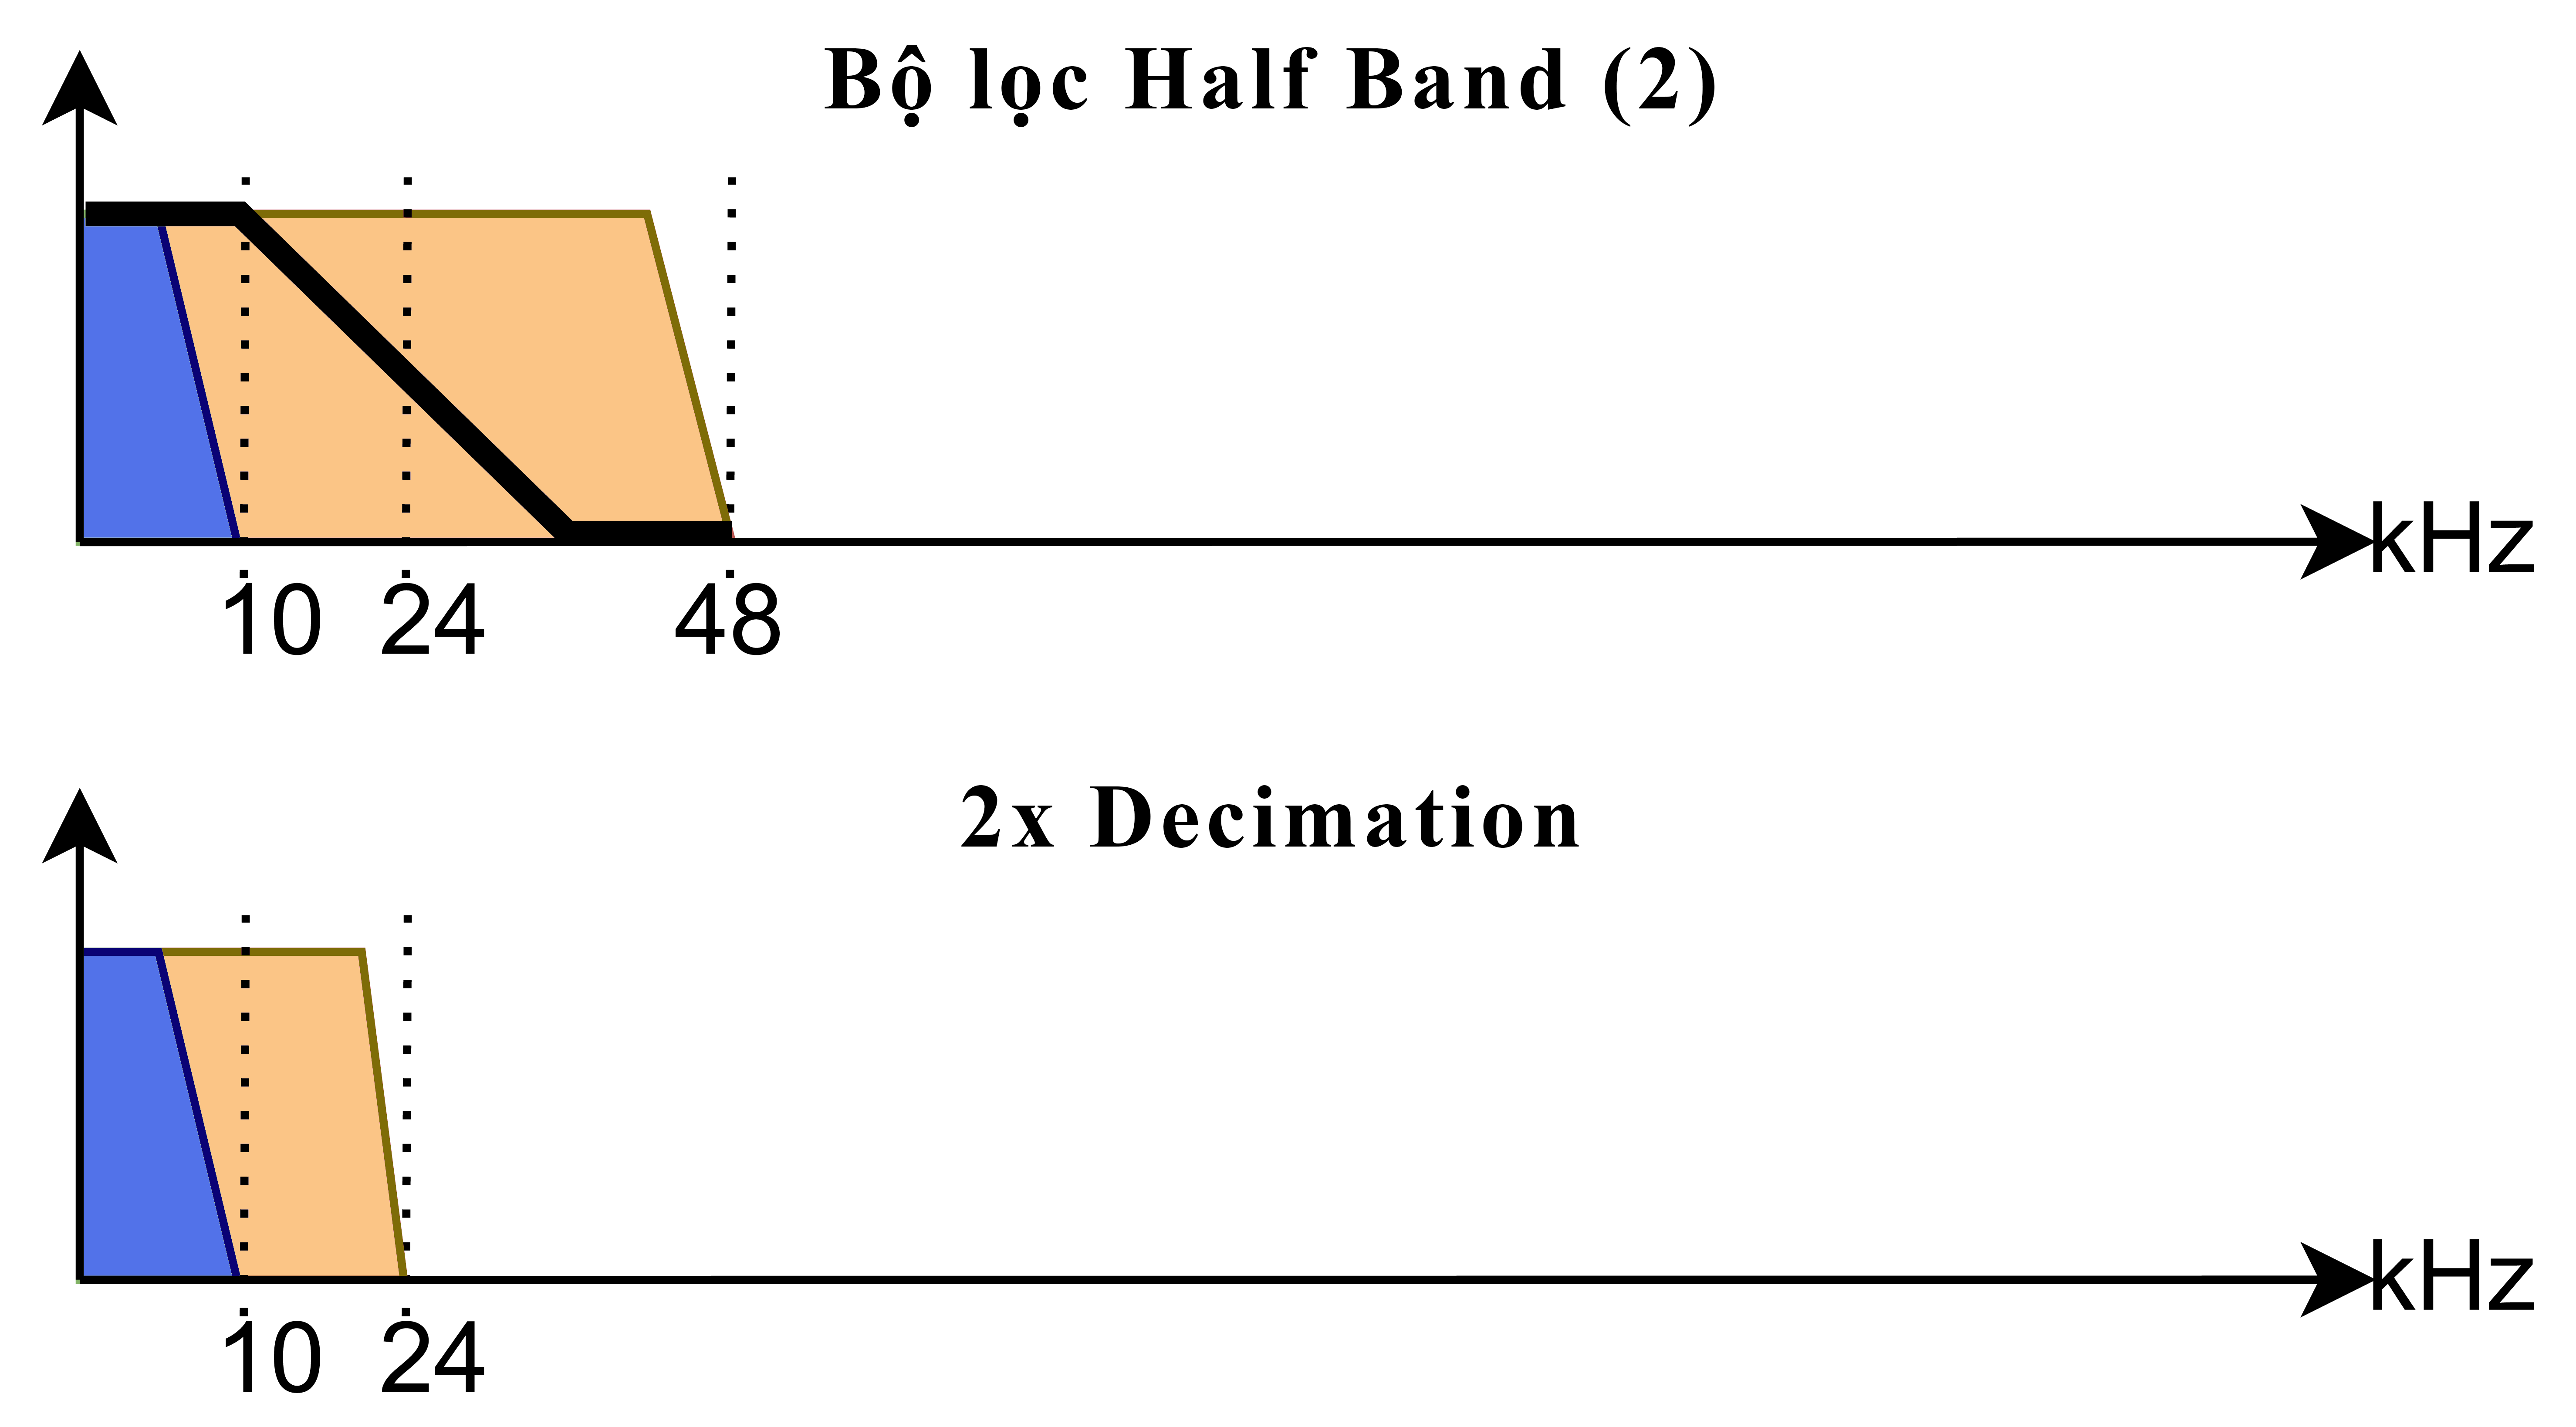
\includegraphics[width=11cm]{Images/Chuong3/3.png}
    \caption[Phổ của tín hiệu sau khi qua bộ lọc Half Band (2) và bộ Decimation 2x]{\bfseries \fontsize{12pt}{0pt}\selectfont Phổ của tín hiệu sau khi qua bộ lọc Half Band (2) và bộ Decimation 2x}
    \label{t3}
\end{figure}
\begin{figure}[H]
    \centering
    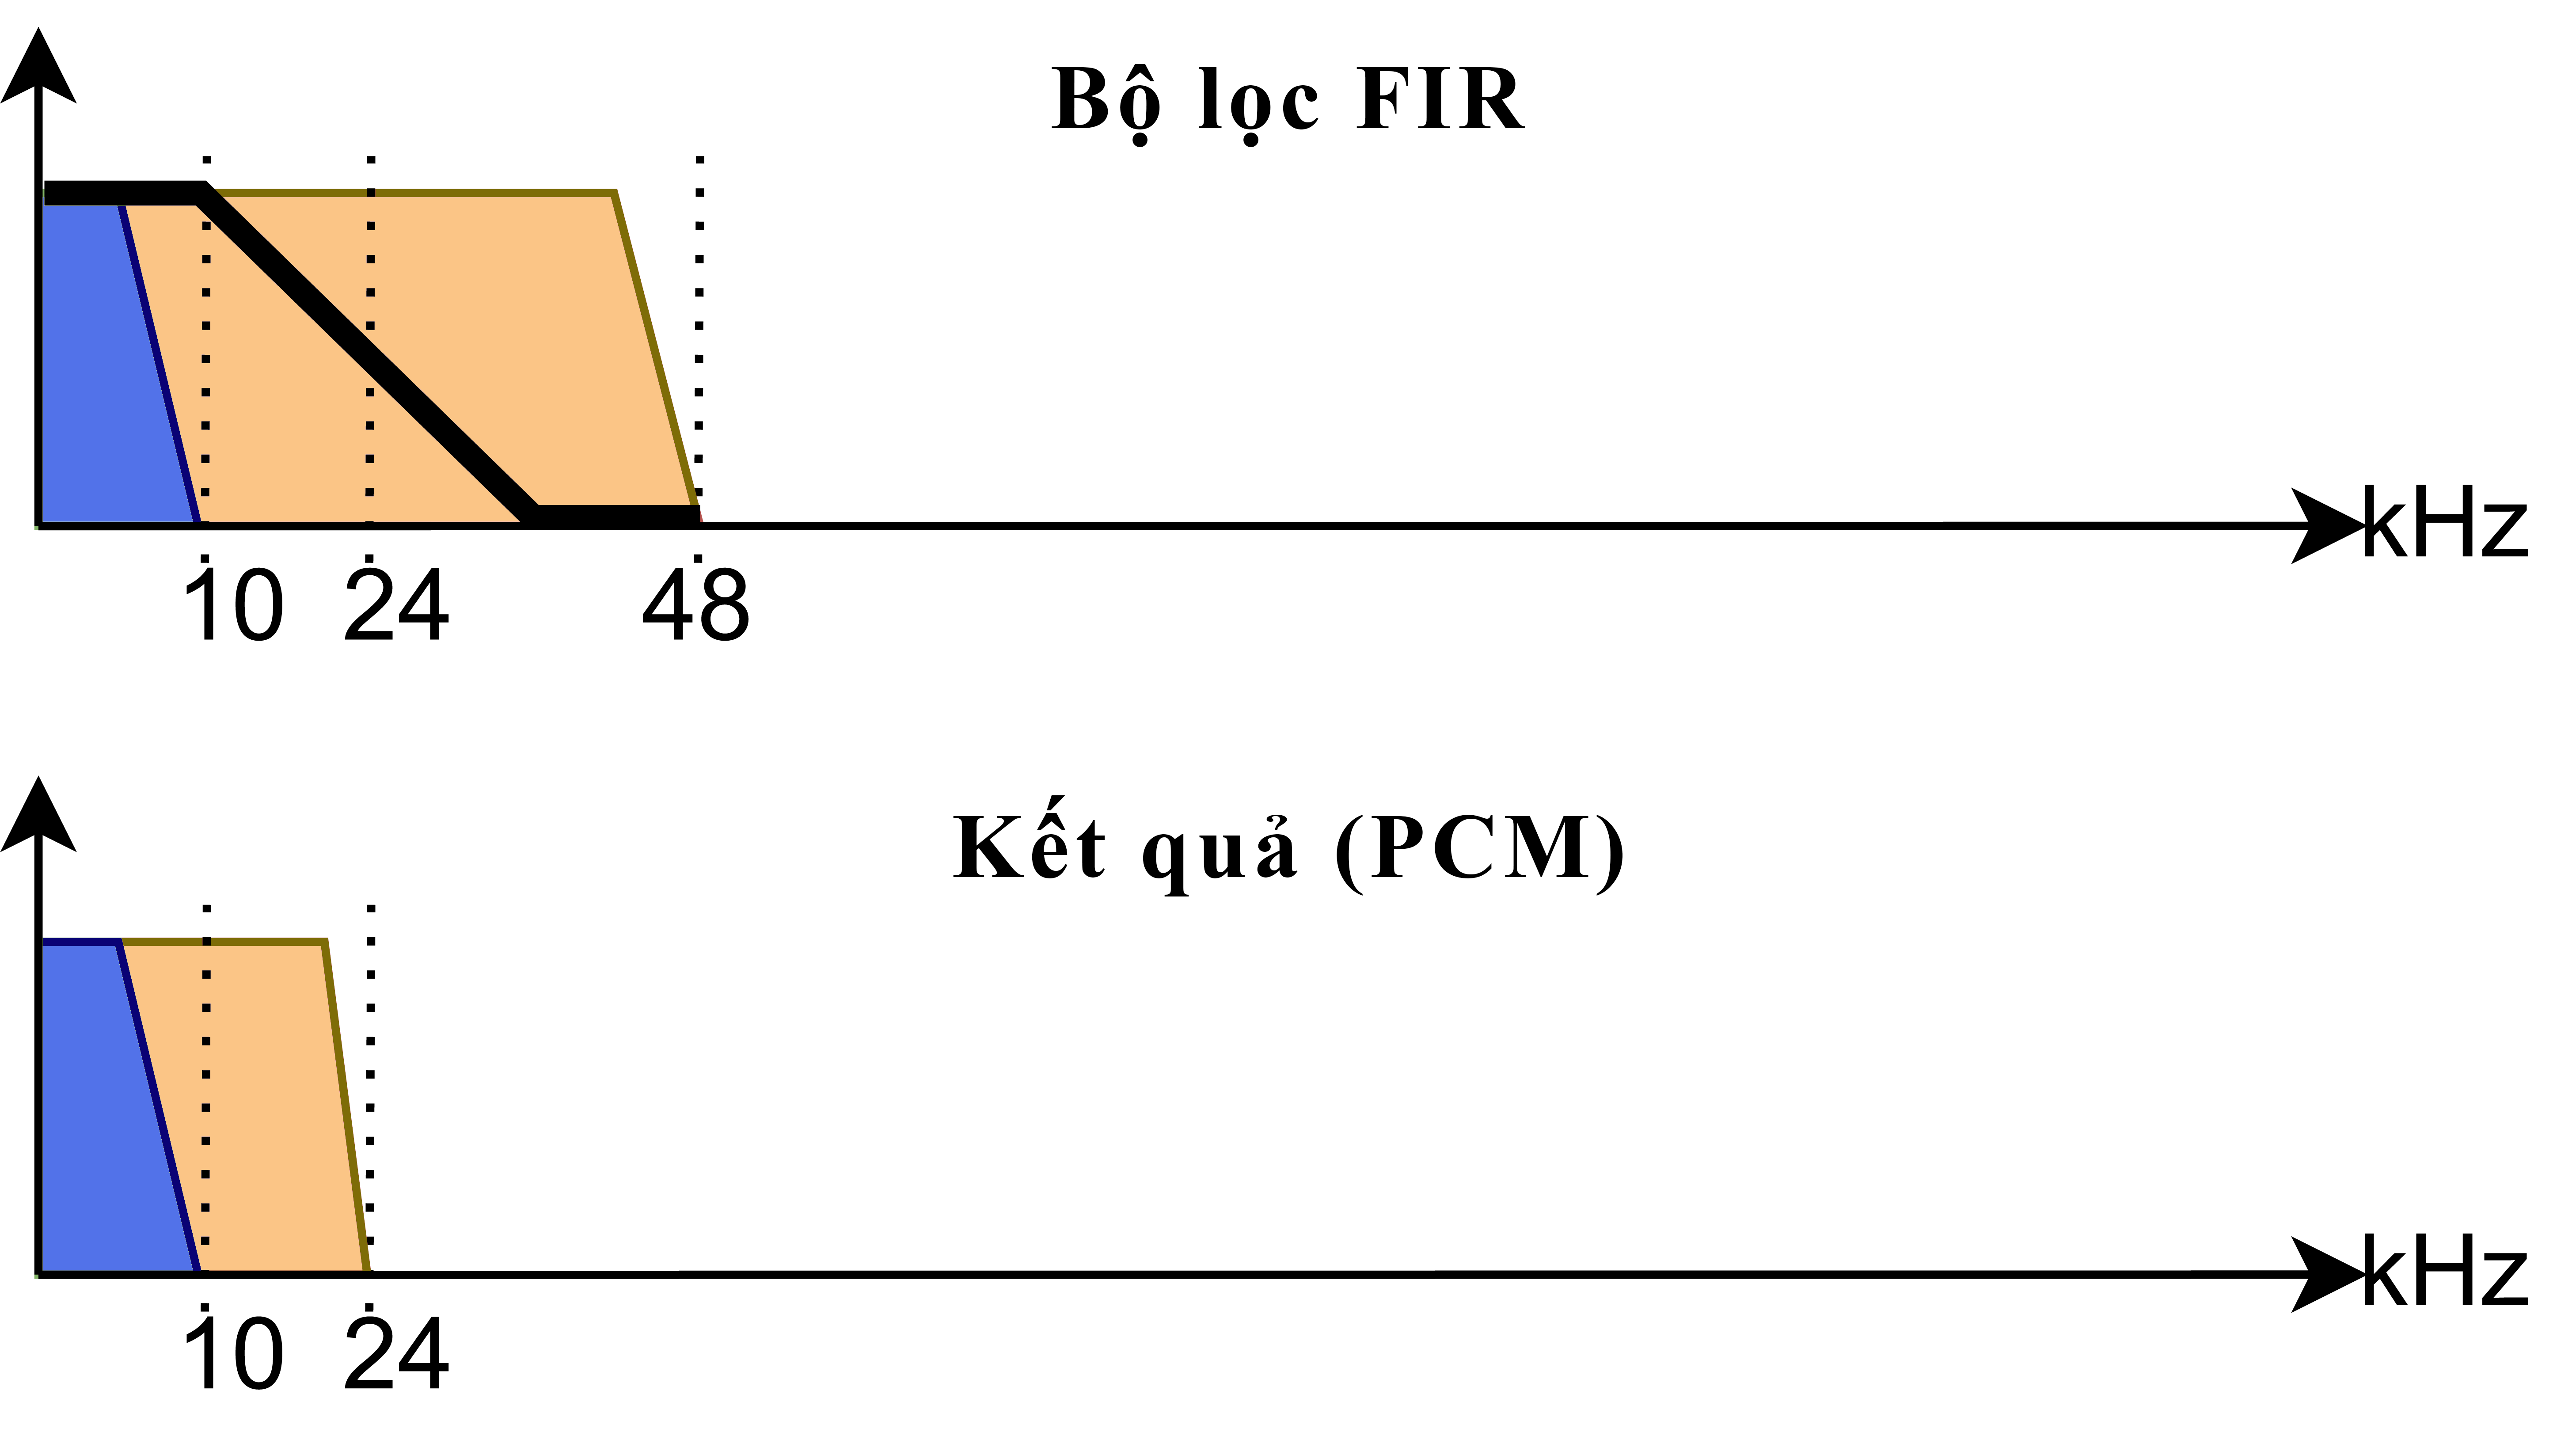
\includegraphics[width=11cm]{Images/Chuong3/4.png}
    \caption[Phổ của tín hiệu thu được cuối cùng]{\bfseries \fontsize{12pt}{0pt}\selectfont Phổ của tín hiệu thu được cuối cùng}
    \label{t4}
\end{figure}

Sau khi chạy thuật toán \textbf{Parks-McClellan/Remez} và tối ưu (mục \ref{toiuu}) với các thông số đã nên ở trên, ta có đồ thị đáp ứng tần số, đáp ứng xung và số lượng taps của từng bộ lọc như hình \ref{a}, \ref{b}, \ref{c}, \ref{d}.  
\vspace{1.5cm}
\begin{figure}[H]
    \centering
    \includesvg[width=15.5cm]{Images/Chuong3/CIC.svg}
    \caption[Đáp ứng tần số và đáp ứng xung của bộ lọc CIC]{\bfseries \fontsize{12pt}{0pt}\selectfont Đáp ứng tần số và đáp ứng xung của bộ lọc CIC}
    \label{a}
\end{figure}
\vspace{1.5cm}
\begin{figure}[H]
    \centering
    \includesvg[width=15.5cm]{Images/Chuong3/HB1.svg}
    \caption[Đáp ứng tần số và đáp ứng xung của bộ lọc Half Band (1)]{\bfseries \fontsize{12pt}{0pt}\selectfont Đáp ứng tần số và đáp ứng xung của bộ lọc Half Band (1)}
    \label{b}
\end{figure}
\vspace{1.5cm}
\begin{figure}[H]
    \centering
    \includesvg[width=15.5cm]{Images/Chuong3/HB2.svg}
    \caption[Đáp ứng tần số và đáp ứng xung của bộ lọc Half Band (2)]{\bfseries \fontsize{12pt}{0pt}\selectfont Đáp ứng tần số và đáp ứng xung của bộ lọc Half Band (2)}
    \label{c}
\end{figure}
\begin{figure}[H]
    \centering
    \includesvg[width=15.5cm]{Images/Chuong3/FIR.svg}
    \caption[Đáp ứng tần số và đáp ứng xung của bộ lọc FIR]{\bfseries \fontsize{12pt}{0pt}\selectfont Đáp ứng tần số và đáp ứng xung của bộ lọc FIR}
    \label{d}
\end{figure}

\noindent \textbf{Nhận xét}: Với tổng số taps bây giờ là 81 (11 + 19 + 51) tương ứng với 81 bộ nhân tối ưu rất nhiều so với 2116 bộ nhân đối với trường hợp đơn giản đã trình bày ở mục \ref{dongian}, tức là giảm hơn 26 lần.
Việc triển khai thiết kế này trên phần cứng sẽ giảm được tài nguyên đáng kể.
\subsection{Mô phỏng và kiểm tra hệ thống}
Việc mô phỏng lại hệ thống sẽ triển khai bằng ngôn ngữ \textbf{Python}, sử dụng thư viện \textbf{Numpy} và \textbf{Scipy}.

Quá trình mô phỏng sẽ được thực hiện như sau: Tín hiệu đầu vào PDM sẽ được chập với đáp ứng xung của từng bộ lọc ở từng giai đoạn. Sau mỗi giai đoạn đó, số mẫu sẽ được giảm đi bằng với tỷ lệ Decimation đã được định sẵn (hình \ref{pipeline_new}).

Để tạo ra tín hiệu PDM, chúng ta phải tiến hành chuyển đổi tín hiệu ban đầu thông qua bộ điều chế Sigma-Delta bậc 4 và tỷ lệ Oversampling 48 bằng thư viện \textbf{deltasigma}.

\textbf{Kiểm tra}:

Cho đầu vào là tín hiệu chứa các thành phần gồm các sóng sin trong dải tần từ 0 - 24 kHz, mỗi thành phần tần số sẽ cách nhau 0.01 kHz và được biểu diễn như phương trình \ref{3sin}.
\begin{equation} \label{3sin}
    x(t) = \frac{0.5}{2400}\sum^{2400}_{f = 1}sin(2\pi \times 100 \times f \times t)
\end{equation}


\begin{figure}[H]
    \centering
    \includesvg[width=16.5cm]{Images/Chuong3/test/pdm_1.svg}
    \caption[Tín hiệu trên miền thời gian sau khi qua bộ điều chế]{\bfseries \fontsize{12pt}{0pt}\selectfont Tín hiệu trên miền thời gian sau khi qua bộ điều chế}
    \label{sd1}
\end{figure}
Tín hiệu này, sau đó sẽ đưa qua bộ điều chế Sigma-Delta. Chúng ta thu được tín hiệu ở miền thời gian và tần số như hình \ref{sd1} và \ref{sd2}.
\begin{figure}[H]
    \centering
    \includesvg[width=16.5cm]{Images/Chuong3/test/psd_3.svg}
    \caption[Phổ mật độ công suất của tín hiệu PDM]{\bfseries \fontsize{12pt}{0pt}\selectfont Phổ mật độ công suất của tín hiệu PDM}
    \label{sd2}
\end{figure}

Hình \ref{sd1} mô tả tín hiệu đầu vào là đường màu đỏ và đường xanh là tín hiệu PDM sau khi được điều chế. Điều chúng ta cần quan tâm ở đây là phổ của tín hiệu PDM (\ref{sd2}). Chúng ta có thể dễ dàng quan sát được, khu vực hình chữ nhật ở đầu tiên (đến đường nét đứt màu xanh lá cây) là tín hiệu các sóng sin từ 0 - 24 kHz  (có thể quan sát rõ ràng ở hình \ref{sd3}), đây là khu vực chúng ta cần quan tâm. Nhiễu lượng tử được đẩy sang miền tần số cao tách biệt với khu vực tần số chứa thông tin.

\begin{figure}[H]
    \centering
    \includesvg[width=16.5cm]{Images/Chuong3/test/psd_2.svg}
    \caption[Phổ mật độ công suất của tín hiệu PDM (2)]{\bfseries \fontsize{12pt}{0pt}\selectfont Phổ mật độ công suất của tín hiệu PDM (2)}
    \label{sd3}
\end{figure}

Vì biên độ các sóng sin đưa vào là bằng nhau. Nên chúng ta có thể do độ suy hao trước và sau khi mô phỏng ở từng dải tần để làm điều kiện nhận xét yêu cầu thiết kế (độ suy hao giải dừng, độ gợn sóng dải thông).

Tiến hành mô phỏng, thu được tín hiệu ở bộ lọc FIR cuối cùng có biểu đồ ở miền thời gian như hình \ref{pcm_o}. Về miền thời gian, chúng ta sẽ rất khó để nhận xét được thiết kế đã đáp ứng được yêu cầu đặt ra hay chưa. Vì vậy, để nhận xét kỹ hơn, hãy quan sát biểu đồ mật độ công suất của tín hiệu PCM đầu ra.
\begin{figure}[H]
    \centering
    \includesvg[width=14cm]{Images/Chuong3/test/pcm_o.svg}
    \caption[Tín hiệu thu được sau mô phỏng]{\bfseries \fontsize{12pt}{0pt}\selectfont Tín hiệu thu được sau mô phỏng}
    \label{pcm_o}
\end{figure}

Hình \ref{psd_pcm} mô tả phổ của tín hiệu đầu ra của hệ thống. Có thể thấy, bắt đầu từ điểm 6 kHz các thành tần số bắt đầu suy giảm mạnh. Độ suy hao của các cách thành phần tần số trong trong miền 0 - 6 kHz ổn định ở mức -73.7193 dB (hình \ref{psd_pcm}). Quay về với phổ PDM ban đầu (hình \ref{sd3}), độ suy hao là -73.6202 dB. Độ chênh lệch 0.0991 dB đã đáp ứng đúng thông số độ gợn sóng của dải thông yêu cầu (0.1 dB). 
\begin{figure}[H]
    \centering
    \includesvg[width=16.5cm]{Images/Chuong3/test/psd_pcm.svg}
    \caption[Phổ của tín hiệu thu được (PCM)]{\bfseries \fontsize{12pt}{0pt}\selectfont Phổ của tín hiệu thu được (PCM)}
    \label{psd_pcm}
\end{figure}

Ở điểm 10 kHz, đồ thị bắt đầu biến thiên nhỏ hơn. Cho nên đây là điểm bắt đầu của dải dừng và kết thúc dải thông. Ở dải tần số này (10 kHz - 24 kHz), độ suy hao cao nhất là 164.8165 dB. Nó chênh lệch so với suy hao ban đầu của PDM đầu vào là 91.1963 dB (164.8165 dB - 73.6202 dB) và đây được coi là độ suy hao của dải dừng, trong khi hệ thống chỉ yêu cầu độ suy hao dải dừng là 89 dB.

\textbf{Kết luận}: Hệ thống đã hoạt động đúng với yêu cầu thiết kế đã đặt ra. Các thành phần tần số không muốn được xem đã được loại bỏ. Tín hiệu trong khoảng tần số từ 0 - 6 kHz đã được lọc chính xác.


\subsection{Kết luận chương}

Qua \hyperref[chuong3]{chương 3}, chúng ta đã tiến hành chọn và thiết kế kiến trúc cho các bộ lọc trong hệ thống chuyển đổi nhiều giai đoạn. Việc mô phỏng và kiểm thử cũng cho ra kết quả đúng với yêu cầu đặt ra. Trong chương tiếp theo, chúng ta sẽ triển khai hệ thống trên bằng thiết kế số.
\newpage
